% Template for PLoS
% Version 3.4 January 2017
%
% % % % % % % % % % % % % % % % % % % % % %
%
% -- IMPORTANT NOTE
%
% This template contains comments intended 
% to minimize problems and delays during our production 
% process. Please follow the template instructions
% whenever possible.
%
% % % % % % % % % % % % % % % % % % % % % % % 
%
% Once your paper is accepted for publication, 
% PLEASE REMOVE ALL TRACKED CHANGES in this file 
% and leave only the final text of your manuscript. 
% PLOS recommends the use of latexdiff to track changes during review, as this will help to maintain a clean tex file.
% Visit https://www.ctan.org/pkg/latexdiff?lang=en for info or contact us at latex@plos.org.
%
%
% There are no restrictions on package use within the LaTeX files except that 
% no packages listed in the template may be deleted.
%
% Please do not include colors or graphics in the text.
%
% The manuscript LaTeX source should be contained within a single file (do not use \input, \externaldocument, or similar commands).
%
% % % % % % % % % % % % % % % % % % % % % % %
%
% -- FIGURES AND TABLES
%
% Please include tables/figure captions directly after the paragraph where they are first cited in the text.
%
% DO NOT INCLUDE GRAPHICS IN YOUR MANUSCRIPT
% - Figs should be uploaded separately from your manuscript file. 
% - Figs generated using LaTeX should be extracted and removed from the PDF before submission. 
% - Figs containing multiple panels/subfigures must be combined into one image file before submission.
% For figure citations, please use "Fig" instead of "Figure".
% See http://journals.plos.org/plosone/s/figures for PLOS figure guidelines.
%
% Tables should be cell-based and may not contain:
% - spacing/line breaks within cells to alter layout or alignment
% - do not nest tabular environments (no tabular environments within tabular environments)
% - no graphics or colored text (cell background color/shading OK)
% See http://journals.plos.org/plosone/s/tables for table guidelines.
%
% For tables that exceed the width of the text column, use the adjustwidth environment as illustrated in the example table in text below.
%
% % % % % % % % % % % % % % % % % % % % % % % %
%
% -- EQUATIONS, MATH SYMBOLS, SUBSCRIPTS, AND SUPERSCRIPTS
%
% IMPORTANT
% Below are a few tips to help format your equations and other special characters according to our specifications. For more tips to help reduce the possibility of formatting errors during conversion, please see our LaTeX guidelines at http://journals.plos.org/plosone/s/latex
%
% For inline equations, please be sure to include all portions of an equation in the math environment.  For example, x$^2$ is incorrect; this should be formatted as $x^2$ (or $\mathrm{x}^2$ if the romanized font is desired).
%
% Do not include text that is not math in the math environment. For example, CO2 should be written as CO\textsubscript{2} instead of CO$_2$.
%
% Please add line breaks to long display equations when possible in order to fit size of the column. 
%
% For inline equations, please do not include punctuation (commas, etc) within the math environment unless this is part of the equation.
%
% When adding superscript or subscripts outside of brackets/braces, please group using {}.  For example, change "[U(D,E,\gamma)]^2" to "{[U(D,E,\gamma)]}^2". 
%
% Do not use \cal for caligraphic font.  Instead, use \mathcal{}
%
% % % % % % % % % % % % % % % % % % % % % % % % 
%
% Please contact latex@plos.org with any questions.
%
% % % % % % % % % % % % % % % % % % % % % % % %

\documentclass[10pt,letterpaper]{article}
\usepackage[top=0.85in,left=2.75in,footskip=0.75in]{geometry}

% % % % % % % % % % % % % % % % % % % % % % % %

% Extra symbols added
\usepackage{stix}
%Three part table - I think this is allowed
\usepackage[flushleft]{threeparttable}
%external document referencing - this is not allowed
\usepackage{xr}


% % % % % % % % % % % % % % % % % % % % % % % %


% amsmath and amssymb packages, useful for mathematical formulas and symbols
\usepackage{amsmath,amssymb}

% Use adjustwidth environment to exceed column width (see example table in text)
\usepackage{changepage}

% Use Unicode characters when possible
\usepackage[utf8x]{inputenc}

% textcomp package and marvosym package for additional characters
\usepackage{textcomp,marvosym}

% cite package, to clean up citations in the main text. Do not remove.
\usepackage{cite}

% Use nameref to cite supporting information files (see Supporting Information section for more info)
\usepackage{nameref,hyperref}

% line numbers
\usepackage[right]{lineno}

% ligatures disabled
\usepackage{microtype}
\DisableLigatures[f]{encoding = *, family = * }

% color can be used to apply background shading to table cells only
\usepackage[table]{xcolor}

% array package and thick rules for tables
\usepackage{array}

% create "+" rule type for thick vertical lines
\newcolumntype{+}{!{\vrule width 2pt}}

% create \thickcline for thick horizontal lines of variable length
\newlength\savedwidth
\newcommand\thickcline[1]{%
  \noalign{\global\savedwidth\arrayrulewidth\global\arrayrulewidth 2pt}%
  \cline{#1}%
  \noalign{\vskip\arrayrulewidth}%
  \noalign{\global\arrayrulewidth\savedwidth}%
}

% \thickhline command for thick horizontal lines that span the table
\newcommand\thickhline{\noalign{\global\savedwidth\arrayrulewidth\global\arrayrulewidth 2pt}%
\hline
\noalign{\global\arrayrulewidth\savedwidth}}


% Remove comment for double spacing
%\usepackage{setspace} 
%\doublespacing

% Text layout
\raggedright
\setlength{\parindent}{0.5cm}
\textwidth 5.25in 
\textheight 8.75in

% Bold the 'Fig #' in the caption and separate it from the title/caption with a period
% Captions will be left justified
\usepackage[aboveskip=1pt,labelfont=bf,labelsep=period,justification=raggedright,singlelinecheck=off]{caption}
\renewcommand{\figurename}{Fig}

% Use the PLoS provided BiBTeX style
\bibliographystyle{plos2015}

% Remove brackets from numbering in List of References
\makeatletter
\renewcommand{\@biblabel}[1]{\quad#1.}
\makeatother

% Leave date blank
\date{}

% Header and Footer with logo
\usepackage{lastpage,fancyhdr,graphicx}
\usepackage{epstopdf}
\pagestyle{myheadings}
\pagestyle{fancy}
\fancyhf{}
\setlength{\headheight}{27.023pt}
\lhead{
\includegraphics[width=2.0in]{PLOS-submission.eps}}
\rfoot{\thepage/\pageref{LastPage}}
\renewcommand{\footrule}{\hrule height 2pt \vspace{2mm}}
\fancyheadoffset[L]{2.25in}
\fancyfootoffset[L]{2.25in}
\lfoot{\sf PLOS}

%% Include all macros below

\newcommand{\lorem}{{\bf LOREM}}
\newcommand{\ipsum}{{\bf IPSUM}}

%% END MACROS SECTION


\begin{document}
\vspace*{0.2in}

% Title must be 250 characters or less.
\begin{flushleft}
{\Large
\textbf\newline{Haploid selection, sex ratio bias, and transitions between sex-determination systems} % Please use "sentence case" for title and headings (capitalize only the first word in a title (or heading), the first word in a subtitle (or subheading), and any proper nouns).
}
\newline
% Insert author names, affiliations and corresponding author email (do not include titles, positions, or degrees).
\\
Michael Francis Scott\textsuperscript{1\Yinyang*},
Matthew Miles Osmond\textsuperscript{2\Yinyang},
Sarah Perin Otto\textsuperscript{2}
\\
\bigskip
\textbf{1} UCL Genetics Institute, Department of Genetics, Evolution and Environment, University College London, Gower Street, London WC1E 6BT 
\\
\textbf{2} Department of Zoology, University of British Columbia, \#4200 - 6270 University Boulevard, Vancouver, BC, Canada V6T 1Z4
\\
\bigskip

% Insert additional author notes using the symbols described below. Insert symbol callouts after author names as necessary.
% 
% Remove or comment out the author notes below if they aren't used.
%
% Primary Equal Contribution Note
\Yinyang These authors contributed equally to this work.

% Additional Equal Contribution Note
% Also use this double-dagger symbol for special authorship notes, such as senior authorship.
%\ddag These authors also contributed equally to this work.

% Current address notes
%\textcurrency Current Address: Dept/Program/Center, Institution Name, City, State, Country % change symbol to "\textcurrency a" if more than one current address note
% \textcurrency b Insert second current address 
% \textcurrency c Insert third current address

% Deceased author note
%\dag Deceased

% Group/Consortium Author Note
%\textpilcrow Membership list can be found in the Acknowledgments section.

% Use the asterisk to denote corresponding authorship and provide email address in note below.
* m.f.scott@ucl.ac.uk

\end{flushleft}
% Please keep the abstract below 300 words
%currently 312 words
\section*{Abstract}
Sex-determination systems are remarkably dynamic; many taxa display shifts in the location of sex-determining loci or the evolution of entirely new sex-determining systems. 
Predominant theories for why we observe such transitions generally conclude that novel sex-determining systems are favoured by selection if they equalise the sex ratio or increase linkage with a sexually-antagonistic locus. 
We use population genetic models to extend these theories in two ways: 
(1) We explicitly consider selection on loci very tightly linked to the ancestral sex-determining loci, e.g., within the non-recombining region of the ancestral sex chromosomes. 
Variation at such loci can favour the spread of new sex-determination systems in which the heterogametic sex changes (XY to ZW or ZW to XY) and the new sex-determining region is less closely linked (or unlinked) to the locus under selection, which is not predicted by previous theory. 
(2) We also consider selection upon haploid genotypes either during gametic competition (e.g., pollen/sperm competition) or meiosis (i.e., non-Mendelian segregation), selective processes that typically occur in one sex or the other. 
We find that associations with haploid selected loci can drive transitions between sex determination systems, without requiring sexually-antagonistic selection in diploids. 
Unexpectedly, with haploid selection, transitions between male and female heterogamety can also evolve where linkage with the sex-determining locus is weakened. 
Furthermore, haploid selection in the heterogametic sex can cause sex ratio biases, which may increase or decrease with the spread of new sex chromosomes. 
Thus, we find that transitions between sex-determination systems cannot be simply predicted by selection to equalise the sex ratio. 
Overall, our models reveal that transitions between sex-determination systems, particularly transitions where the heterogametic sex changes, can be driven by loci in previously unpredicted genomic locations that experience selection during diploid and/or haploid phases.
These results predict conditions under which sex-determination systems are likely to be labile and draw novel connections with sex ratio evolution.


% Please keep the Author Summary between 150 and 200 words
% Use first person. PLOS ONE authors please skip this step. 
% Author Summary not valid for PLOS ONE submissions.   
%currently 193 words
\section*{Author summary}
Accumulating evidence indicates that systems of sex determination are strikingly diverse and labile in many clades. 
This poses the question: what drives transitions between sex determination systems? 
Here, we use models to derive conditions under which new sex determination systems spread. 
Prevailing views suggest that new sex determination systems are favoured when they equalize the sex ratio and/or when they are more closely linked to genes that experience differential selection in males and females. 
Our models extends these theories to include selection upon haploid genotypes (meiotic drive or gametic competition), which causes sex ratio biases and occurs differently in males and females. 
Surprisingly, we find that neither force (sex ratio selection nor associations with genes that have sex-specific effects) dominates the spread of new sex determination systems alone. 
Even more unexpectedly, we find that new sex-determining alleles do not necessarily have to arise in closer linkage with genes that are differentially selected in males and females to spread. 
Therefore, our models predict loci in previously unexpected genomic locations and/or experiencing various types of selection (including haploid selection) can now be implicated as drivers of transitions between sex determination systems. 

\linenumbers

% Use "Eq" instead of "Equation" for equation citations.
\section*{Introduction}

\externaldocument{Turnover_plos.tex}
\externaldocument{S1_Appendix.tex}
\externaldocument{S2_Appendix.tex}
\externaldocument{S3_Appendix.tex}


Animals and angiosperms exhibit extremely diverse sex-determination systems (reviewed in~\cite{Bull:1983vi,Charlesworth:2010it,Beukeboom:2014vb,Bachtrog:2014bx}). 
Among species with genetic sex determination of diploid sexes (GSD), some taxa have heterogametic males (XY) and homogametic females (XX), including %non-monotreme? I think monotremes have XY but tonnes of translocations, giving: X1,X2...X6 Y1
mammals and most dioecious plants~\cite{Ming:2011iy}; whereas other taxa have homogametic males (ZZ) and heterogametic females (ZW), including Lepidoptera and birds. 
Within several taxa, the chromosome that harbours the master sex-determining region changes. 
For example, transitions of the master sex-determining gene between chromosomes or the evolution of new master sex-determining genes have occurred in Salmonids~\cite{Li:2011fm,Yano:2012di}, Diptera~\cite{Vicoso:2015hf}, and \textit{Oryzias}~\cite{Myosho:2012fv}.
%Presentation at evolution found neo sex chromosome in birds, doesn't seem to be published or bioRxiv yet (consider pers com.), title: A previously unknown neo-sex chromosome mediates plumage divergence and speciation in hybridizing birds Jason Sardell; Elizabeth Cooper; J. Albert C. Uy. I wonder if this is actually a fusion event though?
In addition, many clades exhibit transitions between male (XY) and female (ZW) heterogamety, including snakes~\cite{Gamble2017}, lizards~\cite{Ezaz:2009tk}, eight of 26 teleost fish families~\cite{Mank:2006bt}, true fruit flies (Tephritids,~\cite{Vicoso:2015hf}, amphibians~\cite{Hillis:1990gu}, the angiosperm genus \textit{Silene}~\cite{Slancarova:2013dq}, the angiosperm family \textit{Salicaceae}~\cite{Pucholt2015,Pucholt2017} and Coleoptera and Hemiptera (plate 2~\cite{Beukeboom:2014vb}).
Indeed, in some cases, both male and female heterogametic sex-determination systems can be found in the same species, as reported in houseflies~\cite{Macdonald1978}, midges~\cite{Thompson1971}, frogs~\cite{Ogata:2007jm}, cichlid fish~\cite{Ser:2010iq}, tilapia~\cite{Lee2004}, sea bass~\cite{Vandeputte2007}, and lab-strains of Zebrafish~\cite{Liew2012,Wilson2014}.
In addition, multiple transitions have occurred between genetic (GSD) and environmental sex-determination (ESD) systems, e.g., in reptiles and fishes~\cite{Conover:1987in,Mank:2006bt,Pokorna:2009ui,Ezaz:2009tk,Pen:2010kk,Holleley:2015hc}.

Predominant theories accounting for the spread of new sex-determination systems by selection involve fitness differences between sexes (e.g., sexually antagonistic selection) or sex ratio selection~\cite{Blaser2012, Beukeboom:2014vb,vanDoorn2014re}. 
%\citet{Bull:1977wt} shows that direct selection on new sex determination loci can allow them to spread and switch between male and female heterogamety. 
van Doorn and Kirkpatrick~\cite{vanDoorn:2007eu,vanDoorn:2010hu} and Muralidhar and Veller~\cite{Muralidhar2018} have shown that new sex-determining loci can be favoured if they arise in close linkage with a locus that experiences sexual antagonism. 
Tighter linkage allows a stronger favourable association to build up between a male-beneficial allele, and a neo-Y chromosome, for example. 
Such associations can favour a new partially-masculinizing or partially-feminizing allele~\cite{Muralidhar2018}, a new master sex-determining gene~\cite{vanDoorn:2007eu}, and transitions between male and female heterogamety (trans-GSD transitions, ZW to XY or XY to ZW~\cite{vanDoorn:2010hu}). 
However, any sexually-antagonistic loci that are more closely linked to the ancestral sex-determination locus will develop similar, favourable associations and are expected to hinder the spread of a new sex-determination system. 

The sex ratio is directly determined by the sex-determination system, and it has therefore been suggested that sex ratio selection is a dominant force in the evolution of sex determination (e.g., Bull, 1983, p 66-67 ~\cite{Bull:1983vi}; Buekeboom and Perrin, 2014, Chapter 7~\cite{Beukeboom:2014vb}). 
`Fisherian' sex ratio selection favours a 1:1 zygotic sex ratio when assuming that males and females are equally costly to produce~\cite{Fisher:1930wy,Charnov:1982wg}.
This follows from the fact that, for an autosomal locus, half of the genetic material is inherited from a male and half from a female~\cite{West:2009we}. 
Thus, if the population sex ratio is biased towards one sex, the average per-individual contribution of genetic material to the next generation from the opposite sex is greater. 
Therefore, a mutant that increases investment in the rarer sex will spread via the higher per-individual contributions made by that sex. 
%The default mode of sex ratio selection is `Fisherian' sex ratio selection, which favours equal investment in male and female offspring \citep[i.e., a 1:1 zygotic sex ratio when assuming that males and females are equally costly to produce,][]{Fisher:1930wy,Charnov:1982wg}. 
%Given that the sex-determination system can directly affect the sex ratio, we might expect Fisherian sex ratio selection to influence the spread of new sex-determination systems. 
In the case of sex-chromosome evolution, Kozielska et al. (2014)~\cite{Kozielska:2010vm} consider systems in which the ancestral sex chromosomes experience meiotic drive (e.g., where driving X or Y chromosomes are inherited disproportionately often), which causes sex ratios to become biased~\cite{Hamilton:1967ts}. 
They find that new, unlinked sex-determining loci (masculinizing or feminizing mutations, i.e., neo-Y or neo-W loci) can then spread, which restore an even sex ratio. 

Here we use mathematical models to find the conditions under which new sex-determination systems spread when individuals experience selection at both diploid and haploid stages. 
Even in animal and plant species that have much larger and more conspicuous diploid phases than haploid phases, many loci experience significant haploid selection through gamete competition and/or meiotic drive~\cite{Mulcahy:1996ha,JOSEPH:2004haa}.
We use the term `meiotic drive' to refer to the biased (non-Mendelian) segregation of genotypes during gamete production (from one parent) and the term `gametic competition' to refer to selection upon haploid genotypes within a gamete/gametophyte pool (potentially from multiple parents); the term `haploid selection' encompasses both processes. 

Segregation distortion provides putative evidence of haploid selection and can sometimes be attributed to meiotic drive and/or gametic competition~\cite{Lalanne2004,Fishman2005,Leppala2008,Leppala2013,Didion2015,Didion2016}.
Where it has been characterized, meiotic drive generally occurs either during the production of male or female gametes only~\cite{Ubeda:2005gw,Lindholm:2016cw}.
Gametic competition is also typically sex specific, occurring primarily among male gametes, because there are typically many more pollen/sperm than required for fertilization.
Gametic competition may be particularly common in plants, in which 60-70\% of all genes are expressed in the male gametophyte, and these genes exhibit stronger signatures of selection than random genes~\cite{Borg:2009jpa,Arunkumar:2013iq,Gossmann:2014dua}.
In addition, artificial selection pressures applied to male gametophytes are known to cause a response to selection (e.g.,~\cite{Hormaza:1996cv,Ravikumar:2003uo,Hedhly:2004iv,Clarke:2004ir}. 
A smaller proportion of genes are thought to be expressed and selected during competition in animal sperm, although precise estimates are uncertain~\cite{Zheng:2001fi,JOSEPH:2004haa,Vibranovski:2010et}. 
Nevertheless, recent studies have demonstrated that sperm competition in animals can alter haploid allele frequencies and increase offspring fitness~\cite{Immler:2014im,Alavioon2017}.

There are various ways by which genes experiencing haploid selection could influence transitions between sex-determination systems. 
If we assume that haploid selection at any particular locus predominantly occurs in one sex (e.g., meiotic drive during spermatogenesis), then such loci experience a form of sex-specific selection. 
In this respect, we might expect that haploid selection would affect transitions between sex-determination systems in a similar manner to sex-specific diploid selection (as explored in~\cite{vanDoorn:2007eu,vanDoorn:2010hu}). 
That is, new masculinizing mutations (neo-Y chromosomes) could be favoured via associations with alleles that are beneficial in the male haploid stage. 
On the other hand, sex ratios can also become biased by linkage between the sex-determining region and a locus that harbours genetic variation in haploid fitness. 
For example, there are several known cases of sex ratio bias caused by sex-linked meiotic drive alleles (Burt, 2006, Chapter 6~\cite{Burt:2006}) or selection among X- and Y-bearing pollen~\cite{Lloyd:1974tz,Conn:1981uw,Stehlik:2005ul,Stehlik:2006to,Field:2012fd,Field:2013cc}. 
It is not immediately clear how the spread of new sex-determination systems would be influenced by the combination of sex ratio biases and associations between haploid selected loci and sex-determining regions. 

We find that the spread of novel sex-determiners is influenced by both Fisherian sex ratio selection and by selection on genetically-associated alleles. 
%We find that sex ratio biases caused by haploid selection can exert Fisherian sex ratio selection upon novel sex-determiners but that their spread is also determined by selection on genetically-associated alleles. 
%Indeed, it is only when haploid-selected loci are tightly linked to the ancestral sex-determining region (and so sex ratio biases are initially large) that we see an asymmetry between selection for XY to ZW transitions and ZW to XY transitions (e.g., because haploid selection in males only causes biased zygotic sex ratios in an ancestrally XY system).
Surprisingly, Fisherian sex ratio selection does not dominate; it is possible for selection on linked alleles to drive turnover between sex-determining systems despite causing increasingly biased sex ratios. 
In addition to considering haploid selection, another novel development in our model is that we consider loci that are in very tight linkage with the ancestral sex-determining region. 
%Because sex-determining loci are often found within a region of suppressed recombination, there can be a significant number of tightly linked loci. 
We find that loci tightly linked with the ancestral sex-determining region can drive transitions in which the heterogametic sex changes, even when the neo-sex-determining locus is less closely linked to loci under selection (either including haploid selection or not). 


%Lorem ipsum dolor sit~\cite{bib1} amet, consectetur adipiscing elit. Curabitur eget porta erat. Morbi consectetur est vel gravida pretium. Suspendisse ut dui eu ante cursus gravida non sed sem. Nullam Eq~(\ref{eq:schemeP}) sapien tellus, commodo id velit id, eleifend volutpat quam. Phasellus mauris velit, dapibus finibus elementum vel, pulvinar non tellus. Nunc pellentesque pretium diam, quis maximus dolor faucibus id.~\cite{bib2} Nunc convallis sodales ante, ut ullamcorper est egestas vitae. Nam sit amet enim ultrices, ultrices elit pulvinar, volutpat risus.

%\begin{eqnarray}
%\label{eq:schemeP}
%	\mathrm{P_Y} = \underbrace{H(Y_n) - H(Y_n|\mathbf{V}^{Y}_{n})}_{S_Y} + \underbrace{H(Y_n|\mathbf{V}^{Y}_{n})- H(Y_n|\mathbf{V}^{X,Y}_{n})}_{T_{X\rightarrow Y}},
%\end{eqnarray}

\section*{Model}

%genetic system
We consider transitions between ancestral and novel sex-determining systems using a three-locus model, each locus having two alleles (Fig \ref{fig:model_outline}). 
Locus \textbf{X} is the ancestral sex-determining region, with alleles $X$ and $Y$ (or $Z$ and $W$).
Locus \textbf{A} is a locus under selection, with alleles $A$ and $a$.
Locus \textbf{M} is a novel sex-determining region, at which the null allele ($M$) is initially fixed in the population such that sex of zygotes is determined by the genotype at the ancestral sex-determining region, \textbf{X}; $XX$ genotypes become females and $XY$ become males (or $ZW$ become females and $ZZ$ become males). 
To evaluate the evolution of new sex-determination systems, we consider the invasion, fixation, maintenance, and/or loss of novel sex-determining alleles ($m$) at the \textbf{M} locus. 
%We only do invasion analytically though (is this sentence still ok?)
We assume that the \textbf{M} locus is epistatically dominant over the \textbf{X} locus such that zygotes with at least one $m$ allele develop as females with probability $k$ and as males with probability $1-k$, regardless of the \textbf{X} locus genotype.
With $k=0$, the $m$ allele is a masculinizer (i.e., a neo-Y) and with $k=1$ the $m$ allele is a feminizer (i.e., a neo-W).
With intermediate $k$, we can interpret $m$ as an environmental sex determination (ESD) allele, such that zygotes develop as females in a proportion ($k$) of the environments they experience. 
%We also analyze a model of maternally-controlled environmental sex-determination, where mothers with at least one $m$ allele produce daughters with probability $k$. 

%%%%%%%%%%%%%%%%%%%%%%%%%%%%%%%%%%%%%%%%%%%%%%%%%%%%%%%%%
%Model Outline
%%%%%%%%%%%%%%%%%%%%%%%%%%%%%%%%%%%%%%%%%%%%%%%%%%%%%%%%%
\begin{figure}[!h]
%\centering
%\centerline{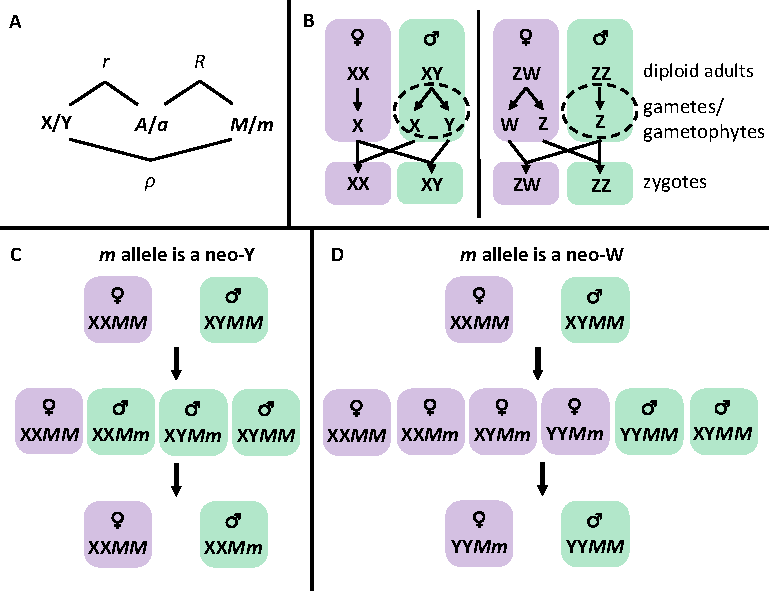
\includegraphics[width=\linewidth]{Sex_determination_outline.pdf}}
\caption{
{\bf Outline of model features.}
Panel A: Recombination rate parameters between the ancestral-sex-determining locus (here, assumed to have X or Y alleles), a locus under selection (\textbf{A}, with alleles $A$ and $a$), and a neo-sex-determining locus (\textbf{M}, with alleles $M$ and $m$). If $r<1/2$, then associations between ancestral-sex-determining alleles (X and Y) and \textbf{A} locus alleles can be maintained past recombination in males. 
Panel B: Haploid selection is often sex-specific, occurring during haploid production or competition in either males or females. 
For example, haploid selection in males only is represented by the dashed circle.  
If X or Y alleles remain associated with alleles that experience haploid selection in males ($r<1/2$), then zygotic sex ratios can become biased because either X or Y male gametes/gametophytes will be abundant after haploid selection. 
However, the zygotic sex ratio is not biased by male haploid selection in ZW sex-determination systems. 
Similarly, zygotic sex ratio biases can occur if haploid selected alleles are associated with neo-sex-determining alleles ($M$ and $m$, i.e., if $R<1/2$). 
Panel C: During cis-GSD transitions (XY to XY or ZW to ZW, without loss of generality we assume ancestral XY sex determination here), a neo-Y allele spreads to pseudo-fixation (its maximum frequency among male gametes) and the the ancestral-Y allele is lost. 
Panel D: During trans-GSD transitions (XY to ZW or ZW to XY), a neo-W allele spreads to pseudo-fixation (its maximum frequency among female gametes) and the ancestral-X allele is lost. Neo-W mutations allow Y-associated alleles into females, which may impede or aid their spread. 
}
\label{fig:model_outline}
\end{figure}
%%%%%%%%%%%%%%%%%%%%%%%%%%%%%%%%%%%%%%%%%%%%%%%%%%%%%%%%%

%life-cycle
In each generation, we census the genotype frequencies in male and female gametes/gametophytes (hereafter gametes) before gametic competition. 
A full description of our model, including recursion equations, is given in \nameref{app:recurs}. 
First, competition occurs among male gametes (sperm/pollen competition) and among female gametes (egg/ovule competition) separately. 
Selection during gametic competition depends on the \textbf{A} locus genotype, relative fitnesses are given by $w_A^\Hermaphrodite$ and $w_a^\Hermaphrodite$ ($\Hermaphrodite \in \{\female,\male\}$; see table \ref{tab:fitnesstable}). %$w_{A}^\male$ and $w_{a}^\male$ for male gametes and $w_{A}^\female$ and $w_{a}^\female$ for female gametes, see table \ref{tab:fitnesstable}. 
We assume that all gametes compete for fertilization during gametic competition, which assumes a polygamous mating system. 
Gametic competition in monogamous mating systems is, however, equivalent to meiotic drive in our model (described below), as either only alters the frequency of gametes produced by heterozygotes. 
After gametic competition, random mating occurs between male and female gametes.
The resulting zygotes develop as males or females, depending on their genotypes at the \textbf{X} and \textbf{M} loci. %(and the \textbf{M} genotype of their mother in the case of maternal control).
Diploid males and females then experience selection, with relative fitnesses $w_{AA}^{\Hermaphrodite}$, $w_{Aa}^{\Hermaphrodite}$, and $w_{aa}^{\Hermaphrodite}$. %where $g$ is the diploid genotype at the \textbf{A} locus ($g \in \{AA, Aa, aa\}$).  
%Diploids compete with others of the same sex, where selection depends on the sex of the individual and its genotype at the \textbf{A} locus.
The next generation of gametes is produced by meiosis, during which recombination and sex-specific meiotic drive can occur. 
Recombination (i.e., an odd number of cross-overs) occurs between loci \textbf{X} and \textbf{A} with probability $r$, between loci \textbf{A} and \textbf{M} with probability $R$, and between loci \textbf{X} and \textbf{M} with probability $\rho$.
Any linear order of the loci can be modelled with appropriate choices of $r$, $R$, and $\rho$ (see Fig \ref{fig:model_outline}A and \nameref{tab:chisubstitutions}). 
Individuals that are heterozygous at the \textbf{A} locus may experience meiotic drive; a gamete produced by $Aa$ heterozgotes of sex $\Hermaphrodite$ bears allele $A$ with probability $\alpha^\Hermaphrodite$. 
Thus, the \textbf{A} locus can experience sex-specific gametic competition, diploid selection, and/or meiotic drive. 

\begin{table}[ht]
%\centering
\smallskip
\caption{{\bf Relative fitness of different genotypes in sex $\Hermaphrodite \in \{\female,\male\}$ } }
\begin{tabular}{l c }
\hline\hline
  Genotype & Relative fitness during gametic competition \\ [0.5ex] \hline
  A & $w_{A}^\Hermaphrodite = 1+t^\Hermaphrodite$ \\
  a & $w_{a}^\Hermaphrodite = 1$ \\ [0.5ex] \hline
  Genotype & Relative fitness during diploid selection \\ [0.5ex] \hline
  AA & $w_{AA}^\Hermaphrodite = 1+ s^\Hermaphrodite$ \\
  Aa & $w_{Aa}^\Hermaphrodite = 1+h^\Hermaphrodite s^\Hermaphrodite$ \\
  aa & $w_{aa}^\Hermaphrodite = 1$ \\ [0.5ex] \hline
  Genotype & Transmission during meiosis in $Aa$ heterozygotes \\ [0.5ex] \hline
  A & $\alpha^\Hermaphrodite=1/2+\alpha_{\Delta}^{\Hermaphrodite}/2$ \\
  a & $1-\alpha^\Hermaphrodite=1/2-\alpha_{\Delta}^{\Hermaphrodite}/2$ \\
  \hline \hline
  \label{tab:fitnesstable}
 \end{tabular}
\end{table}

%%%%%%%%%%%%%%%%%%%%%%%%%%
\section*{Results}
%%%%%%%%%%%%%%%%%%%%%%%%%

The model outlined above describes both ancestrally-XY and ancestrally-ZW sex-determination systems if we relabel the two sexes as being ancestrally `heterogametic' or ancestrally `homogametic'. 
Without loss of generality, we primarily refer to the ancestrally heterogametic sex as male and the ancestrally homogametic sex as female.
That is, we describe an ancestral XY sex-determination system but our model is equally applicable to an ancestral ZW sex-determination system (relabelling the ancestrally-heterogametic sex as female and the ancestrally-homogametic sex as male and switching the labels of males and females throughout). 

\subsection*{Generic invasion by a neo-Y or neo-W}

The evolution of a new sex-determination system requires that a rare mutant allele at the novel sex-determining locus, $m$, increases in frequency when rare. 
The spread of a rare mutant $m$ at the \textbf{M} locus is determined by the leading eigenvalue of the system of eight equations describing the frequency of eggs and sperm carrying the $m$ allele in the next generation (equations \ref{eq:recursions}). %, evaluated at the above equilibrium.
%Thus, the system describing the change in frequency of the $m$ allele consists of eight recursion equations. 
This system simplifies substantially in a number of cases of interest. 
Dominant neo-Y (when $k=0$) or neo-W alleles (when $k=1$) are only found in male diploids (neo-Y) or female diploids (neo-W) such that their growth rate ultimately depends only on the change in frequency of $m$-bearing gametes produced by males or by females, respectively. 
Furthermore, if the $m$ allele is fully epistatically dominant over the ancestral sex-determining system, phenotypes are not affected by the genotype at the ancestral sex-determining region (\textbf{X} locus). 
Thus, the invasion of a rare dominant neo-Y or neo-W allele, $m$, into a system with ancestral sex-determination system $i\in\{XY,ZW\}$ is determined by the largest solution of the quadratic, $(\lambda_m^{(i)})^2+ b \lambda_m^{(i)} + c =0$ \textcolor{blue}{(see \nameref{app:inv_cond} for a discussion of other roots - or Sally's proof!)}.
Here, $b= - (\Lambda_{mA}^{(i)} + \Lambda_{ma}^{(i)})+(\chi_{mA}^{(i)} + \chi_{ma}^{(i)})$ and $c = (\Lambda_{mA}^{(i)} - \chi_{mA}^{(i)}) (\Lambda_{ma}^{(i)} - \chi_{ma}^{(i)}) - \chi_{mA}^{(i)} \chi_{ma}^{(i)}$, where $\Lambda_{mj}^{(i)}$ is the multiplicative growth rate (which we will call the ``haplotypic growth rate'') of the neo-sex determination allele $m$ on background $j\in\{A,a\}$ without accounting for loss due to recombination ($R=0$), and $\chi_{mj}$ is the rate at which mutant haplotypes on background $j\in\{A,a\}$ recombine onto the other \textbf{A} locus background in heterozygotes (see Table \ref{tab:haplotype_growth}).
To differentiate between the invasion of neo-Y and neo-W alleles we write $m=Y'$ or $m=W'$, respectively (e.g., $\Lambda_{W'A}^{(XY)}$ is the growth rate of neo-W alleles on the $A$ background in an ancestral XY system when $R=0$).
The $\Lambda_{mj}^{(i)}$ and $\chi_{mj}^{(i)}$, and thus the spread of the mutant $m$ allele, depend on the frequency of alleles at the \textbf{A} and \textbf{X} loci in the ancestral population. 
In the ancestral population, it is convenient to follow the frequency of the $A$ allele among female gametes (eggs), $p^\female_X$, and among X-bearing, $p^\male_X$, and among Y-bearing, $p^\male_Y$, male gametes (sperm/pollen). 
We also track the fraction of male gametes that are Y-bearing, $q$, which may deviate from $1/2$ due to meiotic drive in males. 
We will consider only equilibrium frequencies of alleles, $\hat{p}^\Hermaphrodite_i$, and Y-bearing male gametes, $\hat{q}$, when calculating the eigenvalues.  

\begin{table}[!ht]
\centering
\smallskip
%\caption{Parameters determining invasion (equation \ref{eq:charpoly_neoY}) for neo-Y or neo-W alleles}
\caption{ {\bf Parameters determining invasion of mutant neo-Y and neo-W alleles into an ancestrally XY system}}
\begin{tabular}{l}
\hline\hline
   \noalign{\vskip 0.5ex}
   $m$ is a neo-Y ($k=0$) \\ [0.5ex] \hline \noalign{\vskip 1ex}
  $\Lambda_{Y'A}^{(XY)} = {\left( 2 \zeta \right)}^{-1} \left[\hat{p}_X^\female w_{A}^{\female} w_{A}^{\male} w_{AA}^{\male} + (1-\hat{p}_X^\female) w_{a}^{\female} w_{A}^{\male} w_{Aa}^{\male} (1+\alpha_{\Delta}^{\male}) \right]/ \left( \bar{w}_H^\female \bar{w}_H^\male \bar{w}^{\male}_{D} \right) $\\ [0.5ex] \noalign{\vskip 0.5ex}
  $\Lambda_{Y'a}^{(XY)} = {\left( 2 \zeta \right)}^{-1} \left[(1-\hat{p}_X^\female) w_{a}^{\female} w_{a}^{\male} w_{aa}^{\male} + \hat{p}_X^\female w_{A}^{\female} w_{a}^{\male} w_{Aa}^{\male}(1 - \alpha_{\Delta}^{\male}) \right]/ \left( \bar{w}_H^\female \bar{w}_H^\male \bar{w}^{\male}_{D} \right) $ \\ [0.5ex] \noalign{\vskip 0.5ex}
  $\chi_{Y'A}^{(XY)} = R {\left( 2 \zeta \right)}^{-1} \left[ (1-\hat{p}_X^\female) w_{a}^{\female} w_{A}^{\male} w_{Aa}^{\male} (1+\alpha_{\Delta}^{\male}) \right]/  \left( \bar{w}_H^\female \bar{w}_H^\male \bar{w}^{\male}_{D} \right)   $\\ [0.5ex] \noalign{\vskip 0.5ex}
  $\chi_{Y'a}^{(XY)} = R {\left( 2 \zeta \right)}^{-1} \left[   \hat{p}_X^\female w_{A}^{\female} w_{a}^{\male} w_{Aa}^{\male} (1 - \alpha_\Delta^{\male}) \right]/ \left( \bar{w}_H^\female \bar{w}_H^\male \bar{w}^{\male}_{D} \right)  $\\ [1ex] \hline 
  \noalign{\vskip 0.5ex}
  $m$ is a neo-W ($k=1$) \\ [0.5ex] \hline \noalign{\vskip 1ex}
  $\Lambda_{W'A}^{(XY)} = {\left[ 2 (1 - \zeta) \right]}^{-1} \left[ \bar{p}^{\male} w_{A}^{\male} w_{A}^{\female} w_{AA}^{\female}+(1-\bar{p}^{\male}) w_{a}^{\male} w_{A}^{\female} w_{Aa}^{\female}(1+\alpha_{\Delta}^{\female})\right]/ \left(\bar{w}_H^\female \bar{w}_H^\male \bar{w}^{\female}_{D} \right) $ \\ [0.5ex] \noalign{\vskip 0.5ex}
  $\Lambda_{W'a}^{(XY)} = {\left[ 2 (1 - \zeta) \right]}^{-1} \left[ (1-\bar{p}^{\male}) w_{a}^{\male} w_{a}^{\female} w_{aa}^{\female}+\bar{p}^{\male} w_{A}^{\male} w_{a}^{\female} w_{Aa}^{\female}(1-\alpha_{\Delta}^{\female})\right] / \left(\bar{w}_H^\female \bar{w}_H^\male \bar{w}^{\female}_{D} \right) $ \\ [0.5ex] \noalign{\vskip 0.5ex}
  $\chi_{W'A}^{(XY)} = R {\left[ 2 (1 - \zeta) \right]}^{-1} \left[ (1-\bar{p}^{\male}) w_{a}^{\male} w_{A}^{\female} w_{Aa}^{\female} (1+\alpha_{\Delta}^{\female}) \right] / \left(\bar{w}_H^\female \bar{w}_H^\male \bar{w}^{\female}_{D} \right)  $\\ [0.5ex] \noalign{\vskip 0.5ex}
  $\chi_{W'a}^{(XY)} = R {\left[ 2 (1 - \zeta) \right]}^{-1} \left[ \bar{p}^{\male} w_{A}^{\male} w_{a}^{\female} w_{Aa}^{\female} (1-\alpha_{\Delta}^{\female}) \right] / \left(\bar{w}_H^\female \bar{w}_H^\male \bar{w}^{\female}_{D} \right) $ \\ [1ex]
  \hline \hline 
   \end{tabular}
   \begin{flushleft} 
$\bar{p}^{\male}=(1-\hat{q})\hat{p}_X^\male + \hat{q}\hat{p}_Y^\male$ is the average frequency of the $A$ allele among X- and Y-bearing male gametes.
%      \item $R$ is the probability of recombination between loci \textbf{A} and \textbf{M}.
$\zeta$ is the zygotic sex ratio (fraction male).
$\bar{w}^{\Hermaphrodite}_{D}$ is the mean fitness of diploids of sex $\Hermaphrodite$.
$\bar{w}_H^\Hermaphrodite$ is the mean fitness of haploids from sex $\Hermaphrodite$, see \nameref{tab:meanfitnesses}.
\end{flushleft}
  \label{tab:haplotype_growth}
\end{table}

We are particularly concerned with the conditions under which a rare neo-sex-determining allele increases in frequency, which occurs when the largest eigenvalue is greater than one. 
%If the average change in frequency of the two haplotypes that carry the $m$ allele ($Am$ and $am$) is positive, invasion will always occur, i.e., if $(\Lambda_{mA} + \Lambda_{ma})/2 > 1$ then $\Lambda > 1$. 
The leading eigenvalue is the largest solution of $f(\lambda_m^{(i)})=(\lambda_m^{(i)})^2+b\lambda_m^{(i)}+c=0$ and the Perron-Frobenius theorem guarantees that it is positive, unique, and real.  
Since $f(\Lambda_{mA}^{(i)})$ and $f(\Lambda_{ma}^{(i)})$ are of opposite signs, the leading eigenvalue must fall between these two quantities and is the larger of them when $R = 0$ (see \nameref{file:Mathematica}).  
Consequently, if both $\Lambda_{mA}^{(i)}$ and $\Lambda_{ma}^{(i)}$ are greater than one, then the leading eigenvalue will always be greater than one, regardless of the linkage between the neo-sex determination factor and the selected locus ($R$). 
In particular, having $\Lambda_{mA}^{(i)} >1$ and $\Lambda_{ma}^{(i)}>1$ thus guarantees that an unlinked sex determining factor can invade ($R=1/2$).  
Conversely, if both $\Lambda_{mA}^{(i)}$ and $\Lambda_{ma}^{(i)}$ are smaller than one, then invasion can never occur.  
Finally, if only one of  $\Lambda_{mA}^{(i)}$ and $\Lambda_{ma}^{(i)}$ is greater than one, the new sex determining factor can always invade when tightly linked to the selected locus ($R$ near 0).  
Furthermore, it can be shown that the leading eigenvalue declines with $R$, and invasion requires that $R$ is sufficiently small that the following condition holds: 
\begin{equation}\label{eq:lambdasGen}
%\frac{\chi_{mA}}{\Lambda_{mA}-1}+\frac{\chi_{ma}}{\Lambda_{ma}-1}>0.
\chi_{ma}^{(i)}/\left(\Lambda_{ma}^{(i)} - 1\right) + \chi_{mA}^{(i)}/\left(\Lambda_{mA}^{(i)} - 1\right) < 1.
\end{equation}
\noindent 
This condition may or may not be satisfied for the full range of locations of the new sex determining factor, including $R=1/2$, depending on the nature of selection.  
Interpreting this condition, if we assume that only the $mA$ haplotype has a positive growth rate when $R=0$, $\Lambda_{ma}^{(i)}<1<\Lambda_{mA}^{(i)}$, the first term on the left-hand side of \eqref{eq:lambdasGen} is negative and invasion requires that the $mA$ haplotype growth rate ($\Lambda_{mA}^{(i)} - 1$) and the rate at which they are produced by recombination in $ma$ haplotypes ($\chi_{ma}^{(i)}$) are sufficiently large relative to the $ma$ haplotype rate of decline ($1-\Lambda_{ma}^{(i)}$) and the rate of loss of $mA$ haplotypes due to recombination ($\chi_{mA}^{(i)}$).

We can draw a number of key points about the invasion of neo-Y and neo-W mutations from Table \ref{tab:haplotype_growth}. 
First, Fisherian sex ratio selection will favour the spread of a neo-Y if the ancestral zygotic sex ratio is biased towards females, $\zeta<1/2$ (i.e., the first factor of the $\Lambda_{mi}^{(i)}$ is greater than one for a neo-Y and less than one for a neo-W).
However, the spread of a neo-Y (neo-W) also depends on the male (female) fitness of associated alleles (see terms involving equilibrium allele frequencies, $\hat{p}$'s).
Second, invasion by a neo-Y (neo-W) allele does not directly depend on the fitness of female (male) diploids. %(for a given set of equilibrium allele frequencies).
This is because a dominant neo-Y (neo-W) is always found in males (females), and therefore the frequency of the neo-Y (neo-W) allele, $m$, only changes in males (females), Fig \ref{fig:model_outline}C,D. 
Finally, invasions by a neo-Y and a neo-W are qualitatively different.
This is because a gamete with the neo-Y always pairs with a female gamete containing an X, and develop into males, Fig \ref{fig:model_outline}C.
By contrast, a gamete with a neo-W can pair with an X or Y male gamete, developing into a female, Fig \ref{fig:model_outline}D.
Consequently, neo-W bearing females obtain a differerent frequency of $A$ alleles from mating (when $\hat{p}_X^\male \neq \hat{p}_Y^\male$) compared to ancestral ($MM$) females.

In order to explicitly determine the conditions under which a rare neo-sex-determining allele spreads, we must calculate the equilibrium frequency of the $A$ allele (i.e., $\hat{p}^\female_X$, $\hat{p}^\male_X$, and $\hat{p}^\male_Y$) and Y-bearing male gametes ($\hat{q}$) in the ancestral population. 
Since only the \textbf{A} locus experiences selection directly, any deterministic evolution requires that there is a polymorphism at the \textbf{A} locus. 
Polymorphisms can be maintained by mutation-selection balance or transiently present during the spread of beneficial alleles. However, polymorphisms maintained by selection can maintain alleles at intermediate allele frequencies for longer periods. 
Here, we focus on polymorphisms maintained by selection, where the $A$ allele reaches a stable intermediate equilibrium frequency under the ancestral sex-determination system before the neo-sex-determining allele ($m$) arises. 
Such polymorphisms can be maintained by heterozygote advantage, sexually-antagonistic selection, ploidally-antagonistic selection, or a combination~\cite{Immler:2012tl}.
We can analytically calculate the allele frequency of the $A$ allele using two alternative simplifying assumptions: 
(1) the \textbf{A} locus is within (or tightly linked to) the non-recombining region around the ancestral SDR ($r \approx 0$) or (2) selection is weak relative to recombination ($s^\Hermaphrodite$, $t^\Hermaphrodite$, $\alpha_{\Delta}^\Hermaphrodite$ of order $\epsilon<<1$). 

\subsection*{Tight linkage with the ancestral sex-determining region ($r \approx 0$)}

The ancestral equilibrium allele frequencies and their stability conditions are given in \nameref{app:eq_stab}. 
When there is complete linkage between the ancestral sex-determining region and the \textbf{A} locus ($r=0$), either the $A$ allele or the $a$ allele must be fixed on the Y. 
% because selection on the Y is effectively haploid an incapably of maintaining a polymorphism in the absence of frequency dependent selection. 
Because the labelling of alleles is arbitrary, we will assume that the $a$ locus is fixed on the Y ($p^\male_Y=0$), without loss of generality. 
If there are two alleles maintained at the \textbf{A} locus, the X can either be fixed for the $A$ allele ($\hat{p}^\female_X=\hat{p}^\male_X=1$) or polymorphic (0<$\hat{p}^\female_X, \hat{p}^\male_X$<1). 
%However, because the X is present in both males and females, there are distinct selection pressures on X's in females and X's in males, which will always be paired with an $A$ allele from the Y. 

We find that a neo-Y can never invade an ancestral XY system that already has tight linkage with the locus under selection ($\lambda_{Y'}^{(XY)} \leq 1$ when $r=0$, for details see \nameref{file:Mathematica}). 
When $R=0$, a neo-Y haplotype with the same allele as the ancestral Y is neutral ($\Lambda_{Y'a}^{(XY)}=1$) and does not change in frequency.
The other neo-Y haplotype will not spread ($\Lambda_{Y'A}^{(XY)}<1$) given that the initial equilibrium is stable. 
Therefore, a neo-Y mutation cannot spread in an ancestral XY system ($\lambda_{Y'}^{(XY)} \leq 1$, regardless of $R$) where selected loci are within or very near the non-recombining region around the SDR.
In essence, through tight linkage with the \textbf{A} locus, the ancestral Y becomes strongly specialized on the allele that has the highest fitness across male haploid and diploid phases. 
Given that the ancestral Y is at this equilibrium, it is not possible for a neo-Y to create males that have higher fitness than the ancestral Y. 

Neo-W alleles, on the other hand, can invade an ancestral XY system under some conditions (the full invasion conditions are given in \nameref{app:inv_cond}; equations \ref{Binvasion} and \ref{Ainvasion}). 
Counterintuitively, selection on loci within the non-recombining region of the SDR can favour the invasion of a less closely linked neo-W, whatever the form of selection maintaining a polymorphism (sexually-antagonistic selection, overdominance, ploidally-antagonistic selection, or some combination, Fig \ref{fig:SexAntagTighter}, \nameref{fig:temporalOverdominance}, \nameref{fig:regionPloidAntag}, and \nameref{fig:SexAntagTighterMaleDrive}).  
The conditions become more restrictive, however, with increasing recombination ($R$) between the new sex determining region and the selected locus.  
The invasion of completely unlinked neo-W alleles ($R = 1/2$) can occur with overdominance in males or with haploid selection but is not possible with only sexually-antagonistic selection if selection is directional in each diploid sex (see \nameref{file:Mathematica}).
To develop an intuition for how less closely linked neo-W alleles invade ($R>r$), we first focus on cases where there is no haploid selection and discuss the additional effect of haploid selection in \nameref{app:inv_cond}. 

%%%%%%%%%%%%%%%%%%%%%%%%%%%%%%%%%%%%%%%%%%%%%%%%%%%%%%%%%
%Tighter linkage allows looser sex-linkage to evolve, even in absence of haploid selection
%%%%%%%%%%%%%%%%%%%%%%%%%%%%%%%%%%%%%%%%%%%%%%%%%%%%%%%%%
\begin{figure}[!h]
\centering
%\centerline{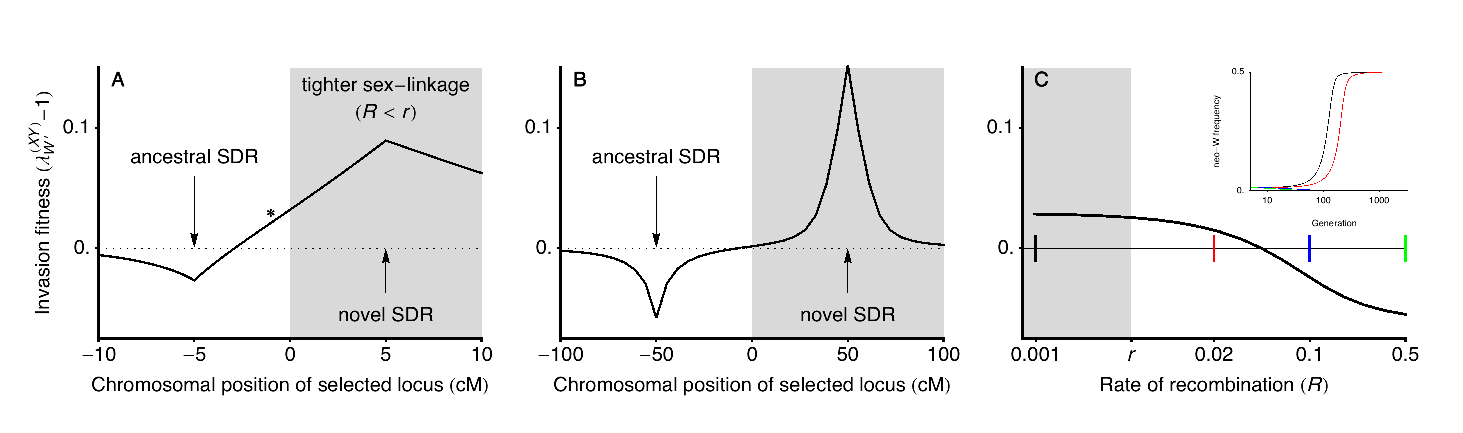
\includegraphics[width=1.5\linewidth]{PositionPlot_SexAntagTighter}}
\caption{
{\bf Transitions between XY and ZW systems can occur even when the neo-SDR is less tightly linked to a locus under sexually-antagonistic selection (here, without haploid selection).}
In panel A, linkage is loose enough relative to selection that the analytical results assuming weak selection hold, and a neo-W can only invade when it is more tightly linked with the selected locus ($R<r$; shaded region).
In panel B, linkage is tight enough relative to selection that the analytical results assuming weak selection do not hold, and a neo-W can invade even when it is less tightly linked with the selected locus ($r<R$; unshaded region marked by \text{*}).
In panel C we vary the recombination rate between the neo-W and the selected locus ($R$) for a fixed recombination rate between the ancestral-SDR and the selected locus ($r=0.005$). 
Coloured markers show recombination rates for which the temporal dynamics of invasion are plotted in the inset, demonstrating that neo-W alleles can reach pseudo-fixation if they are more (black) or less (red) closely linked to a locus experiencing sexually-antagonistic selection. 
A very loosely linked neo-W does not spread in this case (blue and green lines overlap and go to 0). 
Fitness parameters are: $w_{AA}^\female = 1.05$, $w_{aa}^\male = 1.2$, $w_{aa}^\female = w_{AA}^\male = 0.85$, $w_{Aa}^\Hermaphrodite = 1$,  $t^\Hermaphrodite = \alpha^\Hermaphrodite_\Delta = 0$.
%\textcolor{red}{consider removing panel A, which is repeated in Fig 3.}
%\textcolor{blue}{probably better to remove from panel 3, eh?}
}
\label{fig:SexAntagTighter}
\end{figure}
%%%%%%%%%%%%%%%%%%%%%%%%%%%%%%%%%%%%%%%%%%%%%%%%%%%%%%%%%

If we categorise the $a$ allele as being ancestrally `male-beneficial' via the fact that it is fixed on the Y, then $\Lambda_{W'A}^{(XY)}>1$ indicates that the neo-W spreads when found with the ancestrally `female-beneficial' allele. 
Broadly, this is possible because the ancestral X chromosome is sometimes found in males and is therefore unable to perfectly specialise on the `female-beneficial' allele. 
For example, when the $a$ allele is favoured on the ancestral X in males, a polymorphism of $A$ and $a$ alleles can be maintained on the X despite selection for the $A$ allele in females ($s^\female>0$, $0<h^\female<1$), see outlined region in Fig \ref{fig:regionplots}A. 
When the $a$ allele is strongly favoured on X chromosomes in males ($w_{aa}^\male$ sufficiently large relative to $w_{Aa}^\male$), neo-W-$A$ haplotypes can spread ($\Lambda_{W'A}^{(XY)}>1$, see grey region in Fig \ref{fig:regionplots}A) because they produce hgher fitness females ($AA$ or $Aa$ genotypes) and are unleashed from counterselection in males. 

%%%%%%%%%%%%%%%%%%%%%%%%%%%%%%%%%%%%%%%%%%%%%%%%%%%%%%%%%
%Both neo-W haplotypes can spread, in the absence of haploid selection, when there is overdominance
%%%%%%%%%%%%%%%%%%%%%%%%%%%%%%%%%%%%%%%%%%%%%%%%%%%%%%%%%
\begin{figure}[!h]
\centering
%\centerline{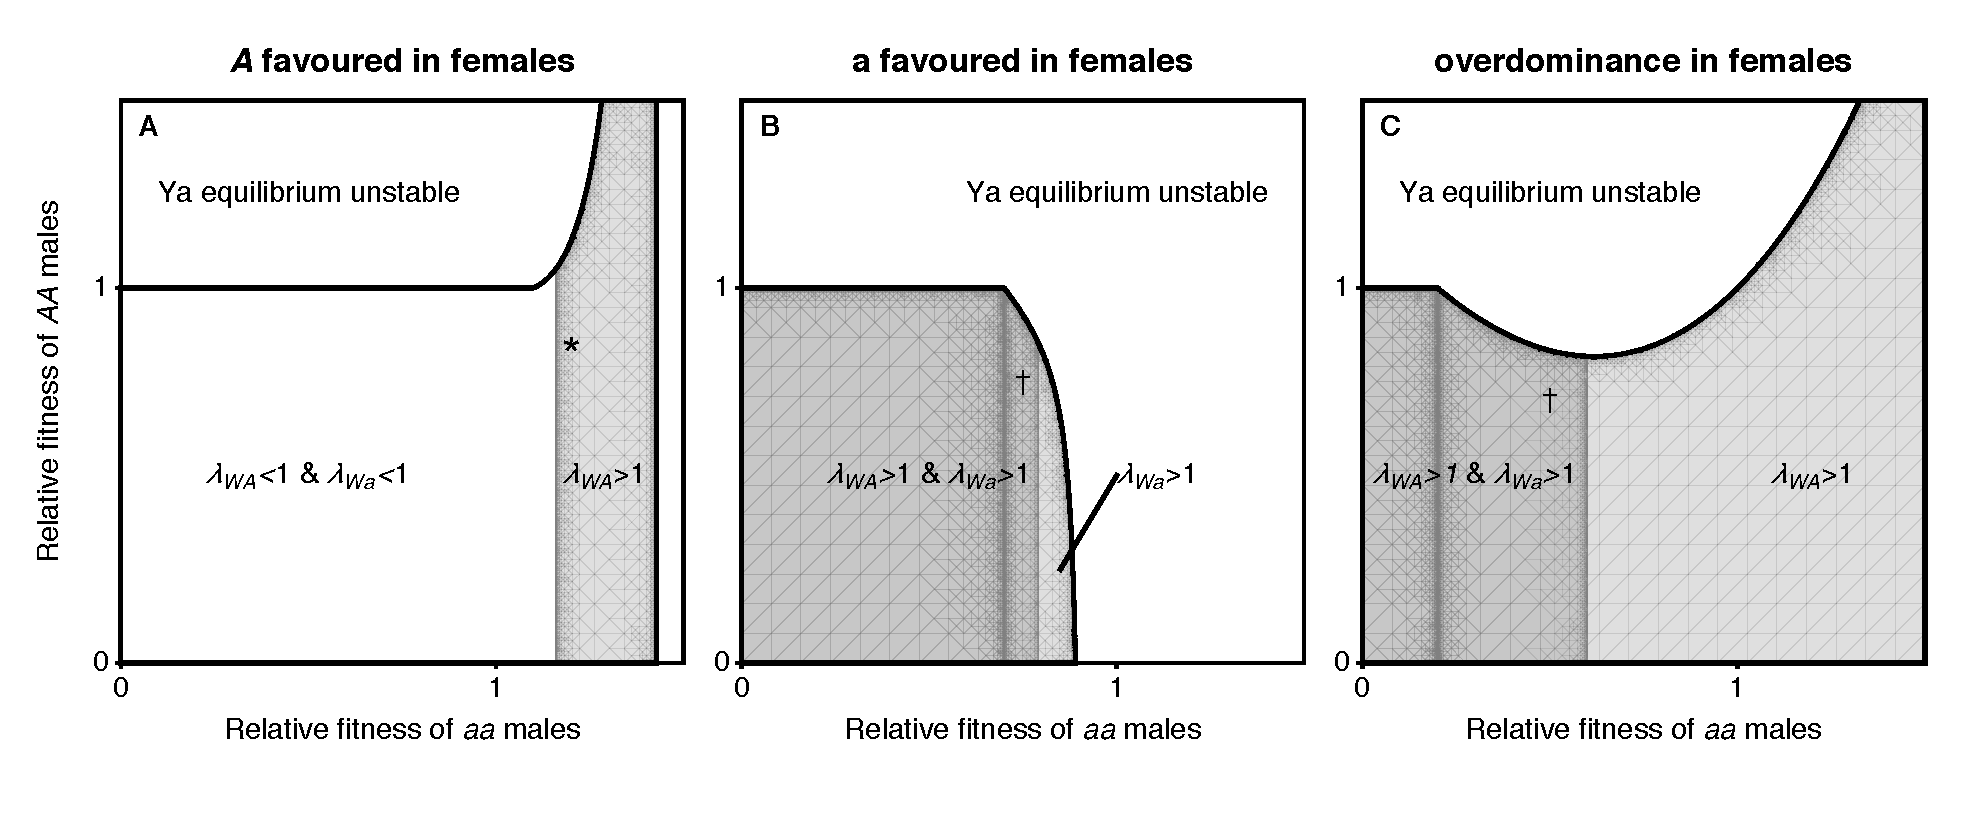
\includegraphics[width=1.25\linewidth]{Region_plot_combined_Mike}}
%\centerline{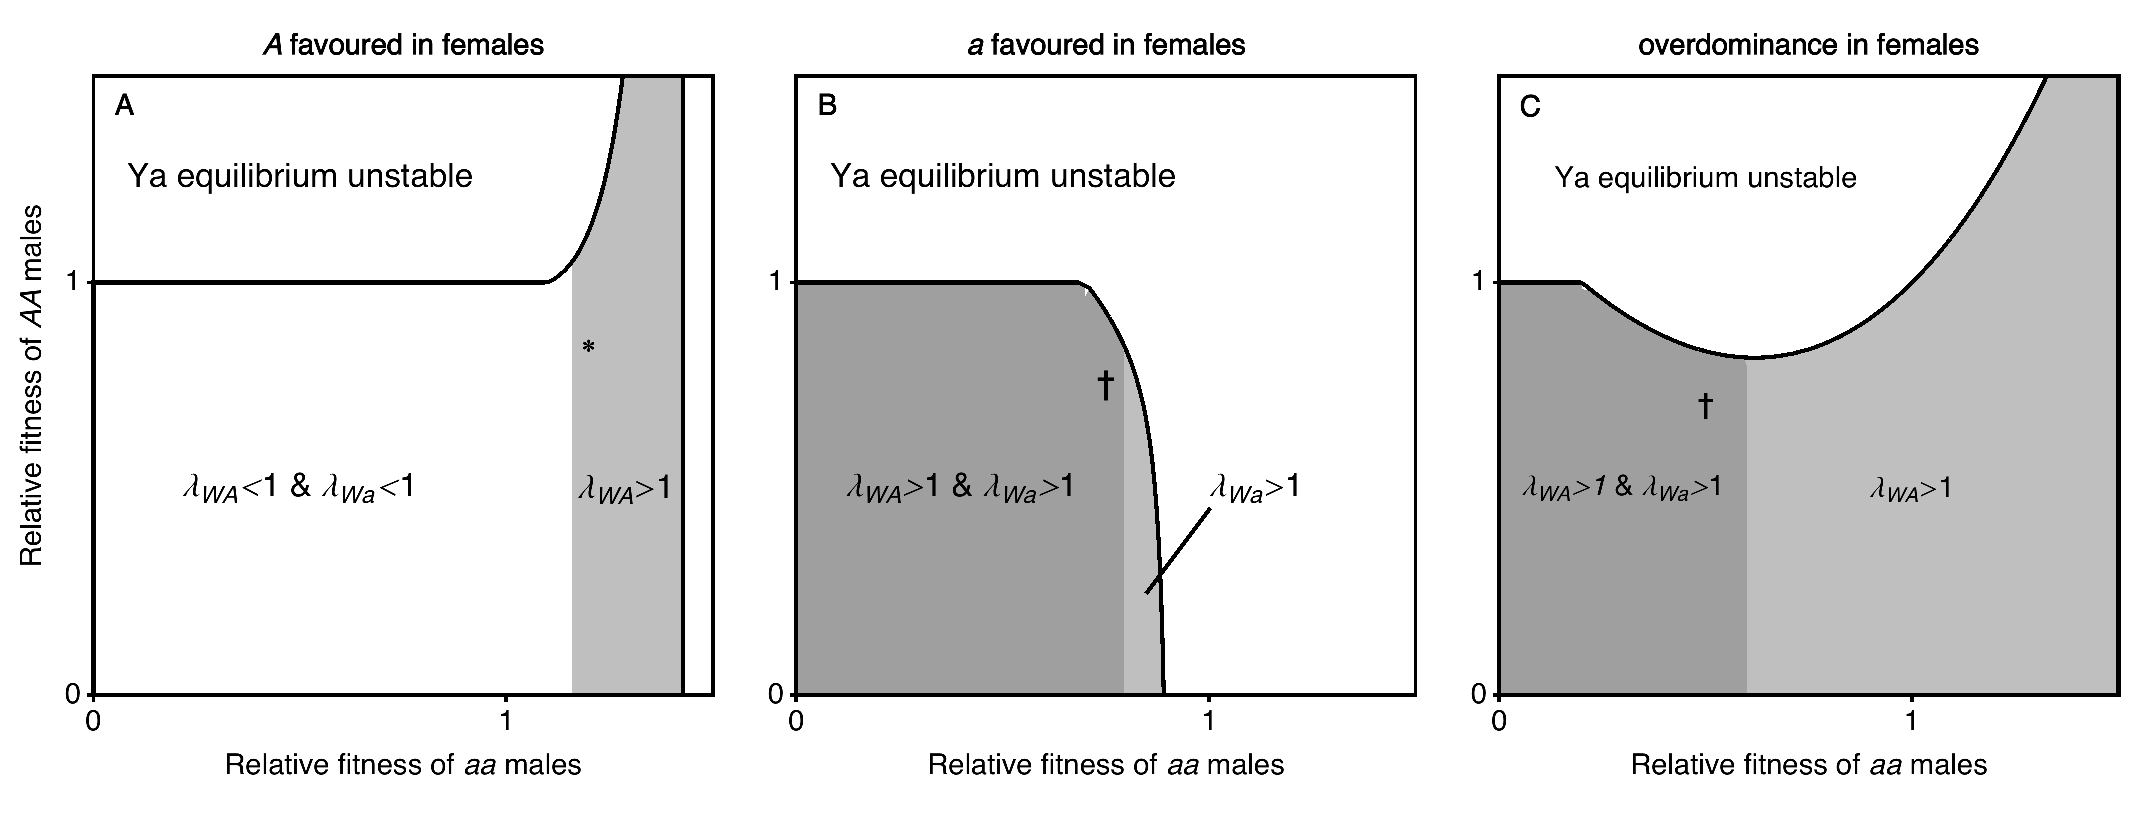
\includegraphics[width=1.25\linewidth]{Region_plot_combined}}
\caption{
{\bf When the ancestral-XY locus is tightly linked to a locus under selection ($r=0$), one or both neo-W haplotypes can spread. }
We vary the fitness of male homozygotes relative to heterozygotes ($w_{Aa}^\Hermaphrodite=1$) and only consider stable equilibria at which both \textbf{A} locus alleles are maintained and the $a$ allele is initially fixed on the Y, region outlined. 
Here, selection in females can favour the $A$ allele (panel A, $w_{aa}^\female=0.85$, $w_{AA}^\female=1.05$), favour the $a$ allele (panel B, $w_{aa}^\female=1.05$, $w_{AA}^\female=0.85$), or be overdominant (panel C, $w_{aa}^\female=w_{AA}^\female=0.6$). 
If $\Lambda_{W'A}^{(XY)}$ or $\Lambda_{W'a}^{(XY)}$ is greater than one, then a rare neo-W can spread for, at least, some values of $R>r$. 
The parameter values marked with an asterisk correspond to the fitnesses used in Fig \ref{fig:SexAntagTighter}C. 
Where both $\Lambda_{W'A}^{(XY)}$ and $\Lambda_{W'a}^{(XY)}$ are greater than one, a neo-W will spread when rare, regardless of linkage with the selected locus (for any $R$). 
\nameref{fig:positionOverdominance} shows the dynamics using the parameters marked with a dagger. 
Here, there is no haploid selection $t^\Hermaphrodite = \alpha^\Hermaphrodite_\Delta = 0$.
}
\label{fig:regionplots}
\end{figure}


%%%%%%%%%%%%%%%%%%%%%%%%%%%%%%%%%%%%%%%


When only one neo-W haplotype has a positive growth rate (see Fig \ref{fig:regionplots}), a neo-W can invade as long as equation \eqref{eq:lambdasGen} is satisfied, which may require that the recombination rate, $R$, is small enough.
Nevertheless, because we assume here that $r$ is small, these results indicate that a more loosely linked sex-determining region ($r<R$) can spread.
For example, tightly sex-linked loci that experience sexually-antagonistic selection can drive trans-GSD transitions in which the neo-SDR is less closely linked to the locus under selection (Fig \ref{fig:SexAntagTighter}). 

Given that the $a$ allele can be considered ancestrally `male-beneficial' because it is fixed on the Y, it is surprising that neo-W-$a$ haplotypes can sometimes be favoured by selection in females ($\Lambda_{W'a}^{(XY)}>1$). 
Again, this occurs because ancestral X's also experience selection in males, in which they will always be paired with a Y-$a$. 
If there is overdominance in males, X-$A$ Y-$a$ males have high fitness and the $A$ allele is favoured by selection on the X in males. 
Therefore, the X can be polymorphic or even fixed for the $A$ allele despite favouring the $a$ allele during selection in females (e.g., see outlined region in Fig \ref{fig:regionplots}B and~\cite{Lloyd1977,Otto2014}). 
In such cases, neo-W-$a$ haplotypes can spread because they create more $Aa$ and $aa$ females when pairing with an X from males and because they bring Y-$a$ haplotypes into females, where it has higher fitness (Fig \ref{fig:model_outline}D). 

In some cases, both W-$A$ and W-$a$ haplotypes can spread, e.g., when $AA$ individuals have low fitness in females yet the $A$ is polymorphic or fixed on the X due to overdominance in males (Fig \ref{fig:regionplots}B and \ref{fig:regionplots}C).
Both neo-W-$A$ and neo-W-$a$ haplotypes then produce fewer unfit $AA$ females.
This is true for the neo-W-$A$ haplotype because it can pair with a Y-$a$ haplotype and still be female. 
Wherever both haplotypes have positive growth rates, invasion by a neo-W is expected regardless of its linkage with the selected locus (i.e., for any $R$, see \nameref{fig:positionOverdominance} and \nameref{fig:temporalOverdominance} for examples). 

Assuming weak selection, van Doorn and Kirkpatrick~\cite{vanDoorn:2010hu} showed that invasion by a neo-W occurs under the same conditions as `pseudo-fixation' (at pseudo-fixation the neo-W reaches its maximum frequency among eggs, which is 1/2). 
An equivalent analysis is not possible where recombination rates are low. 
However, numerical simulations demonstrate that the neo-SDR does not necessarily reach pseudo-fixation, leading to the stable maintenance of a mixed sex-determining system, in which X, Y, Z, and W alleles all segregate (e.g., \nameref{fig:freqAll}B,C). 


\subsection*{Loose linkage with the ancestral sex-determining region}

Here we assume that selection is weak ($s^\Hermaphrodite$, $t^\Hermaphrodite$, $\alpha_{\Delta}^\Hermaphrodite$ of order $\epsilon<<1$) and thus implicitly assume that all recombination rates ($r$, $R$ and $\rho$) are large relative to selection.
%, we denote the leading eigenvalues describing the invasion of a neo-Y ($k=0$) and a neo-W ($k=1$) into an ancestrally XY system by $\lambda_{Y',XY}$ and $\lambda_{W',XY}$, respectively. 
To leading order in selection, the leading eigenvalues are:

\begin{equation}
\lambda_{Y'}^{(XY)} =1+ \frac{1}{4}V_{A}S_{A}^2\frac{ \left( r-R \right) }{r R}+O\left(\epsilon^3 \right) 
\label{eq:lambda_neoY}
\end{equation}

\noindent 
and 

\begin{equation}
\lambda_{W'}^{(XY)} =\lambda_{Y'}^{(XY)}+\left(2\alpha_{\Delta}^\male-2\alpha_{\Delta}^\female+t^\male-t^\female \right) \left( \hat{p}^\male_Y-\hat{p}^\male_X \right)/2
+O\left(\epsilon^3 \right)
\label{eq:lambda_neoW}
\end{equation}

\noindent
where $V_{A}=\bar{p}(1-\bar{p})$ is the variance in the equilibrium frequency of $A$ and $S_{A}=(D^\male +\alpha_{\Delta}^\male+t^\male) - (D^\female+\alpha_{\Delta}^\female+t^\female)$ describes sex differences in selection for the $A$ versus $a$ allele across diploid selection, meiosis, and gametic competition.
The diploid selection term, $D^\Hermaphrodite=\big{[} \bar{p}s^\Hermaphrodite+(1-\bar{p})h^\Hermaphrodite s^\Hermaphrodite\big{]} -\big{[} \bar{p}h^\Hermaphrodite s^\Hermaphrodite+(1-\bar{p}) \big{]}$, is the difference in fitness between $A$ and $a$ alleles in diploids of sex $\Hermaphrodite \in \{\female,\male\}$, where $\bar{p}$ is the leading-order probability of mating with an $A$-bearing gamete from the opposite sex (equation \ref{eq:pAve}). 
The difference in $A$-allele-frequency among Y-bearing sperm versus X-bearing sperm is given by $\hat{p}^\male_Y-\hat{p}^\male_X=V_{A}\big{(}D^\male - D^\female+\alpha_{\Delta}^\male-\alpha_{\Delta}^\female+t^\male-t^\female\big{)}(1-2r)/(2r)$. 

The neo-sex-determining allele, $m$, will spread in an XY system if $\lambda_{m}^{(XY)}>1$. 
Equation \eqref{eq:lambda_neoY} demonstrates that, under weak selection, a neo-Y will invade an XY system if and only if it is more closely linked to the selected locus than the ancestral sex-determining region (i.e., if $R<r$; note that $V_{A}S_{A}^2$ is strictly positive as long as \textbf{A} is polymorphic). 
This echoes our results above where a neo-Y could never invade if $r\approx0$. 
It is also consistent with the results of \cite{vanDoorn:2007eu}, who considered diploid selection only and also found that cis-GSD transitions (XY to XY or ZW to ZW) can only occur when the neo-sex-determining locus is more closely linked to a locus under sexually-antagonistic selection. 
%Because tighter linkage between the sex-determining region and a selected locus evolves during these transitions, stronger associations between selected alleles and diploid sexes can build up by selection (e.g., between male-beneficial alleles and the male-determining allele, Y).%, increasing diploid mean fitness (Fig \ref{fig:Combination_MeanFit}). 

With weak selection and no haploid selection ($t^\Hermaphrodite=\alpha^\Hermaphrodite_{\Delta}=0$), the spread of a neo-W is equivalent to the spread of a neo-Y ($\lambda_{W'}^{(XY)}=\lambda_{Y'}^{(XY)}$), such that trans-GSD transitions (XY to ZW or ZW to XY) can also occur only if the neo-sex-determining region is more closely linked to a locus under selection ($R<r$), as found by \cite{vanDoorn:2010hu}. 
When there is haploid selection, invasion also typically occurs when the neo-W is more closely linked to the selected locus than the ancestral sex-determining region (Fig \ref{fig:Combination_Centimorgans}).
For example, if the \textbf{A} locus is unlinked to the ancestral sex-determining region ($r=1/2$), a more closely linked neo-W ($R<1/2$) can always invade.
In this case, there is no ancestral association between \textbf{A} alleles and sex chromosomes in males, $\left( \hat{p}^\male_Y-\hat{p}^\male_X \right)=0$, see equation \eqref{eq:freq_diffs}. 
The second term in equation \eqref{eq:lambda_neoW} therefore disappears and invasion depends only on the sign of $(r-R)$.%, as in the case of the neo-Y. 

%%%%%%%%%%%%%%%%%%%%%%%%%%%%%%%%%%%%%%%%%%%%%%%%%%%%%%%%%
%A neo-W can invade an XY system under a large number of selective regimes
%%%%%%%%%%%%%%%%%%%%%%%%%%%%%%%%%%%%%%%%%%%%%%%%%%%%%%%%%
\begin{figure}[!h]
\centering
%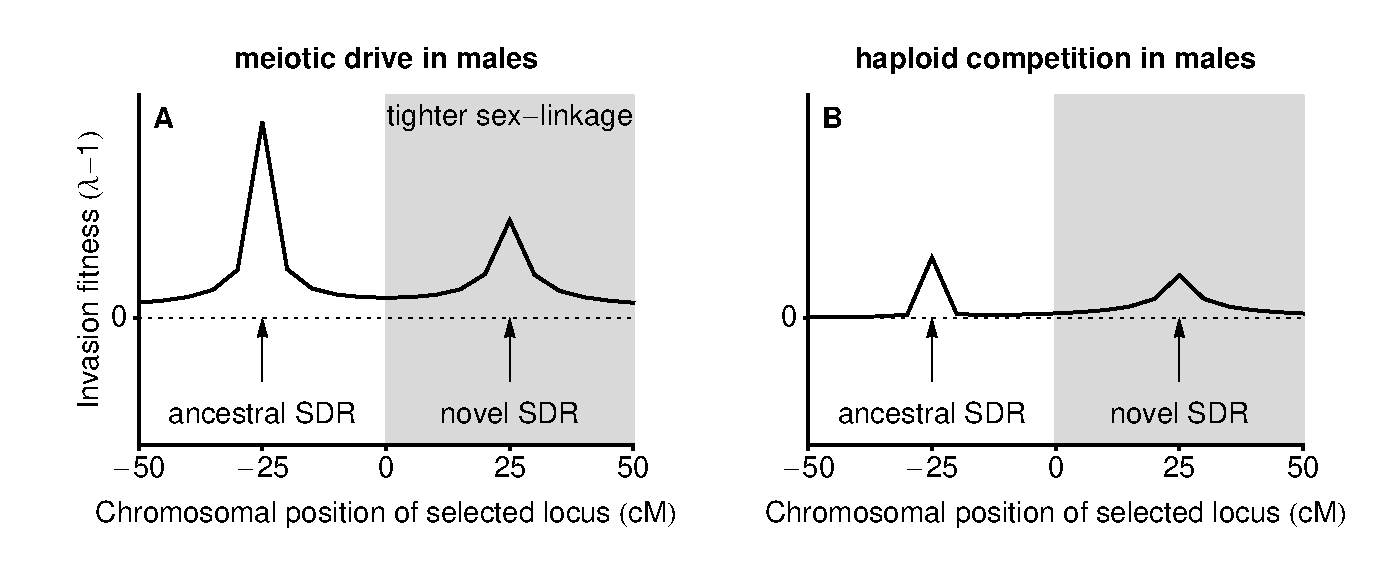
\includegraphics[width=\linewidth]{PositionPlot}
\caption{
{\bf Ploidally-antagonistic selection allows a less tightly linked neo-W to invade.}
In panel A, male drive ($\alpha^\male_{\Delta} = -1/20$, $t^\Hermaphrodite = \alpha^\female_{\Delta} = 0$) opposes selection in diploids (no sex-differences: $s^\Hermaphrodite = 1/10$, $h^\Hermaphrodite = 7/10$), in which case the neo-sex-determining allele can invade regardless of $R$.   
In panel B, gametic competition in males ($t^\male = -1/10$, $t^\female = \alpha^\Hermaphrodite_{\Delta} = 0$) opposes selection in diploids (sex-differences: $s^\male = 3/20$, $s^\female = 1/20$, $h^\Hermaphrodite = 7/10$), in which case the neo-sex-determining allele can once again invade regardless of $R$.
}
\label{fig:Combination_Centimorgans}
\end{figure}
%%%%%%%%%%%%%%%%%%%%%%%%%%%%%%%%%%%%%%%%%%%%%%%%%%%%%%%%%

However, with haploid selection, the additional term in equation \eqref{eq:lambda_neoW} can be positive, which can allow neo-W invasion ($\lambda_{W'}^{(XY)}>1$), even when the neo-sex-determining region is less closely linked to the selected locus ($R>r$). 
%These transitions are unusual because, when $R>r$, associations that selection has built up between alleles more favourable in one sex and alleles that determine sex will be weakened. 
%Mean diploid fitness therefore decreases during heterogametic transitions that create looser sex-linkage (Fig \ref{fig:Combination_MeanFit}B,D). 
%Equation \eqref{eq:lambda_neoW} shows that, with weak selection, neo-W alleles can invade an XY system for a large number of selective regimes. 
%To clarify the parameter space under which $\lambda_{W'}^{(XY)}>1$ , we consider several special cases. 
%Firstly, if the \textbf{A} locus is unlinked to the ancestral sex-determining region ($r=1/2$), a more closely linked neo-W ($R<1/2$) can always invade because there is no ancestral association between $A$ alleles and sex chromosomes in males, $\left( \hat{p}^\male_Y-\hat{p}^\male_X \right)=0$, see equation \eqref{eq:freq_diffs}. 
%The second term in equation \eqref{eq:lambda_neoW} therefore disappears and invasion depends only on the sign of $(r-R)$, as in the case of the neo-Y. 
%Indeed, invasion typically occurs when the neo-W is more closely linked to the selected locus than the ancestral sex-determining region (Fig \ref{fig:Combination_Centimorgans}).
To clarify the parameter space under which invasion occurs despite looser sex-linkage ($\lambda_{W'}^{(XY)}>1$ despite $R>r$), we focus on the special case where $R=1/2$ and $r<1/2$ (e.g., the selected locus is on the ancestral sex chromosome and the novel sex-determining locus arises on an autosome). 
In Table \ref{tab:specialcases} we give the conditions where invasion occurs when we further assume that haploid selection only occurs in one sex (e.g., during male meiosis only) and dominance coefficients are equal in the two sexes, $h^\female=h^\male$. 
When there is no gametic competition and meiotic drive is in one sex only, an unlinked neo-W can invade as long as the same allele is favoured during diploid selection in males and females ($s^\female s^\male>0$, see Fig \ref{fig:Combination_Centimorgans}A and Fig \ref{fig:SexRatioBad}B). %, which is 50\% of the parameter space. 
When there is no meiotic drive and gametic competition occurs in one sex only, an unlinked neo-W can invade as long as the same allele is favoured in male and female diploid selection and there are sex differences in selection of one type (e.g., $s^\female(s^\male-s^\female)>0$, see Fig \ref{fig:Combination_Centimorgans}B). %, which is 25\% of the parameter space. 
These special cases indicate that neo-W invasion occurs for a relatively large fraction of the parameter space, even if the neo-W uncouples the sex-determining locus from a locus under selection. 

\begin{table}[!ht]
\centering
\smallskip
\caption{Invasion conditions for unlinked neo-W ($R=1/2$, $r<1/2$) into ancestral XY with one form of haploid selection}
\begin{tabular}{l l c }
\hline\hline
Scenario &  Assumptions & neo-W spreads ($\lambda_{W'}^{(XY)}>1$) if \\ [0.5ex] \hline
%  $r=1/2$, $R<1/2$ & Always \\ [0.5ex] \hline
%  $r<1/2$, $R=1/2$ &  \\ [0.5ex] \hline
\noalign{\vskip 1mm}
  male drive only & $h^\male=h^\female$, $t^\female=t^\male=\alpha^\female_{\Delta}=0$ & $s^\female s^\male>0$ \\ [0.5ex]
 female drive only & $h^\male=h^\female$, $t^\female=t^\male=\alpha^\male_{\Delta}=0$ & $s^\female s^\male>0$ \\ [0.5ex]
 sperm competition only &  $h^\male=h^\female$, $t^\female=\alpha^\female_{\Delta}=\alpha^\male_{\Delta}=0$ & $s^\female(s^\male-s^\female)>0$ \\ [0.5ex]
  egg competition only & $h^\male=h^\female$, $t^\male=\alpha^\female_{\Delta}=\alpha^\male_{\Delta}=0$ & $s^\male(s^\female-s^\male)>0$ \\ [0.5ex]
  \hline \hline
  \label{tab:specialcases}
 \end{tabular}
\end{table}

%%%%%%%%%%%%%%%%%%%%%%%%%%%%%%%%%%%%%%%%%%%%%%%%%%%%%%%%%
%Sex ratio selection is not a good predictor of neo-W invasion into an XY system
%%%%%%%%%%%%%%%%%%%%%%%%%%%%%%%%%%%%%%%%%%%%%%%%%%%%%%%%%
\begin{figure}[!h]
\centering
%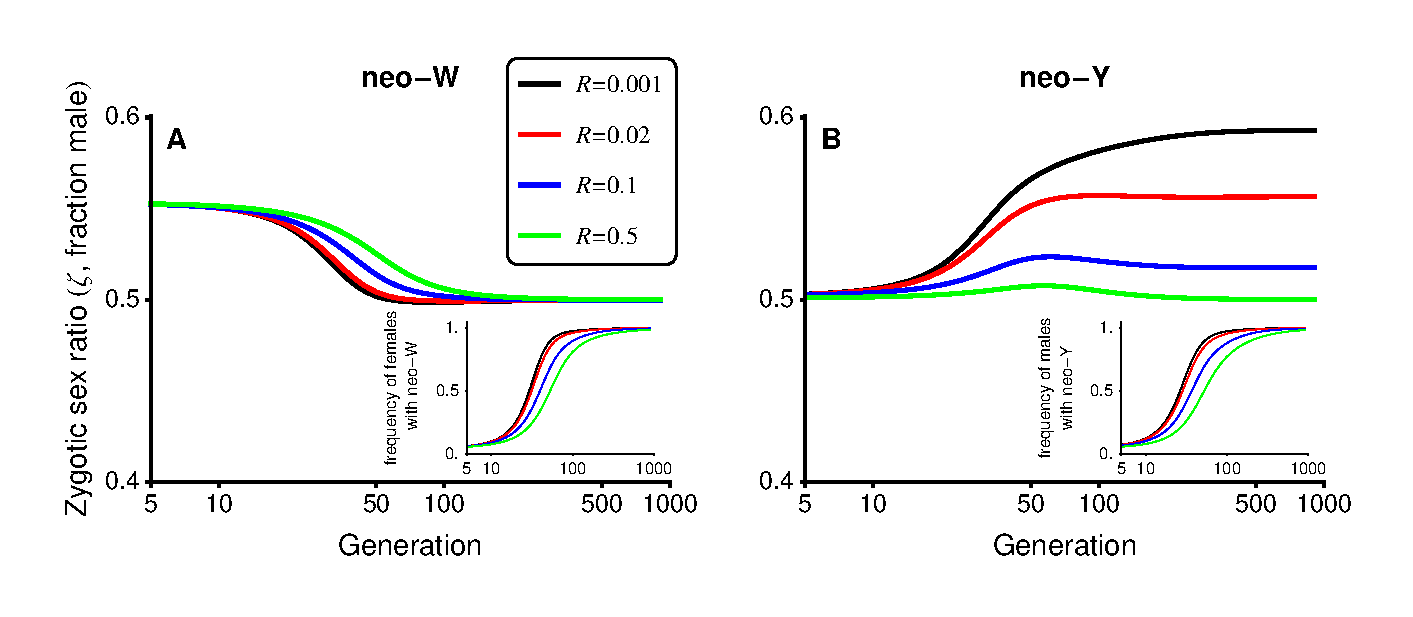
\includegraphics[width=\linewidth]{Temporal_SR}
\caption{
{\bf Fisherian sex ratio selection alone is not a good predictor of turnover between sex-determining systems.}
In this figure, selection is ploidally antagonistic with haploid selection favouring the $a$ allele during male meiosis.
In panel A, male meiotic drive in an ancestral XY system causes a male bias (see Fig \ref{fig:model_outline}B), allowing a neo-W to invade and replace the ancestral sex-determination system (inset shows neo-W frequency among female gametes, reaching pseudo-fixation), which balances the zygotic sex ratio.
In panel B, male drive in an ancestral ZW system has no effect on the zygotic sex ratio yet a neo-Y can invade and replace the ancestral sex-determination system (inset shows neo-Y frequency among male gametes, reaching pseudo-fixation). 
%When $R<1/2$, the neo-Y becomes associated with the allele favoured by drive, causing the zygotic sex ratio to become biased, hence the frequency of the neo-Y at pseudo-fixation can be higher than $0.5$ (inset).
Parameters:  $s^\female =s^\male = 0.2$, $h^\female = h^\male = 0.7$, $t^\female = t^\male = \alpha^\female_\Delta = 0$, $\alpha^\male_\Delta = -0.1$, $r=0.02$.
}
\label{fig:SexRatioBad}
\end{figure}
%%%%%%%%%%%%%%%%%%%%%%%%%%%%%%%%%%%%%%%%%%%%%%%%%%%%%%%%%


Previous research suggests that when the ancestral sex-determining locus is linked to a locus that experiences haploid selection (e.g., meiotic drive), a new, unlinked sex-determining locus invades in order to restore equal sex ratios~\cite{Kozielska:2010vm}. 
Consider, for example, the case where the \textbf{A} locus is linked to the ancestral-SDR ($r<1/2$) and experiences meiotic drive in males only ($\alpha^\male_\Delta \neq 0$, $\alpha^\female_\Delta=0$), without gametic competition ($t^\female=t^\male=0$).
In this case, the zygotic sex ratio can be initially biased only if the ancestral sex-determining system is XY (Fig \ref{fig:model_outline}B and Fig \ref{fig:SexRatioBad}A). 
%If the ancxestral sex-determining system is ZW, the zygotic sex ratio will be 1:1 because diploid sex is determined by the proportion of Z-bearing versus W-bearing eggs and meiosis in females is fair (Fig \ref{fig:Combination_Turnover}D).
If Fisherian sex ratio selection were dominant, we would expect a difference in the potential for XY to ZW and ZW to XY transitions. 
%However, to leading order with selection weak relative to recombination, we find that sex ratio selection favours the spread of a neo-W by an amount equl to the spread of a neo-Y into a ZW system (relabeling XY as the heterogametic sex and reversing the labels of males and females in Table \ref{tab:specialcases})
%However, to leading order with selection weak relative to recombination, we find that sex ratio selection favours the spread of a neo-W (through the first terms in table \ref{tab:haplotype_growth}) by an amount that is equal in magnitude to the fitness effects of alleles associated with new sex-determining alleles (second terms in table \ref{tab:haplotype_growth}).
However, invasion by a neo-W into an XY system and invasion by a neo-Y into a ZW system occur under the same conditions ($\lambda_{Y'}^{(XY)} = \lambda_{W'}^{(XY)}$ and $\lambda_{Y'}^{(XY)}=\lambda_{W'}^{(XY)}$, at least to order $\epsilon^2$).
For example, in Fig \ref{fig:SexRatioBad}A neo-W alleles invade an ancestral-XY system where females are initially rare.
However, Fig \ref{fig:SexRatioBad}B shows that a neo-Y can invade an ancestral-ZW system under the same conditions. 
As a consequence, whenever $R<1/2$, the neo-Y becomes associated with the male meiotic drive allele such that the zygotic sex ratio actually evolves to become biased towards males.

%As selection becomes stronger (or linkage becomes tighter), this symmetry between sex ratio selection and haploid selection is lost, causing differences in the strength of selection favouring the two heterogametic transitions (compare red to black near -25cM and 25 cM in Fig \ref{fig:Combination_Centimorgans}). \textcolor{red}{normalise fitness in sexually antagonistic case}

Why can new sex-determining regions invade when they are more loosely linked to selected loci ($R>r$)?  
Consider first the case where both sex-determining-loci are linked to the selected locus ($r<R<1/2$). 
In an XY system, haploid selection in males can facilitate the spread of a neo-W because the zygotic sex ratio is ancestrally male biased and the W produces more of the rarer sex (Fig \ref{fig:SexRatioBad}A). 
A new sex determining region can also, however, benefit from becoming more associated with drive. 
For example in a ZW system with the same selection regime (haploid selection in males), a neo-Y can spread despite the fact that the zygotic sex is initially even; in this case, the neo-Y spreads because it is often found in males and can, if it carries the driven allele $a$, benefit from haploid selection in males (Fig \ref{fig:SexRatioBad}B). 
While equalizing the sex ratio and benefiting from drive are two primary reasons why haploid selection spurs sex chromosome transitions, more complex situations also arise.  
For example with $R=1/2$ in Fig \ref{fig:SexRatioBad}B (green curve), the neo-Y spreads despite the fact that it cannot benefit from drive because free recombination moves it randomly between driven and non-driven backgrounds.  
Nevertheless, the unlinked neo-Y can spread because diploids bearing it more often carry the non-driven allele $A$, which is found at high frequency on the W background and has higher average diploid fitness to balance the haploid advantage of the $a$ allele at equilibrium.

\subsection*{Environmental sex determination}

We next consider the case where the new sex-determining mutation, $m$, causes sex to be determined probabilistically or by heterogeneous environmental conditions (environmental sex determination, ESD), with individuals carrying allele $m$ developing as females with probability $k$.
Here, we do not assume that the environmental conditions that determine sex also differentially affect the fitness of males versus females. 
Such correlations can favour environmental sex-determination systems that allow each sex to be produced in the environment in which it has highest fitness; in the absence of these correlations, previous theory would predict that ESD is favoured when it produces more equal sex ratios than the ancestral system (see reviews by~\cite{Charnov:1982wg,Bull:1983vi,West:2009we}). %(e.g., maternal condition, mate quality, age, or host size)  

The characteristic polynomial determining the eigenvalues (equations \ref{eq:recursions}) does not factor for ESD mutants as it does for $k=0$ or $k=1$. 
We therefore focus on weak selection here. 
Assuming weak selection, the spread of the new sex-determining region is given by 

\begin{equation}
\begin{split}
\lambda_{ESD'}^{(XY)} =& 1 + \frac{{(1-2k)}^2}{4}V_{A}{S_{A}}^2\frac{r-R}{r R} \\
&+\frac{k(\hat{p}^\male_Y-\hat{p}^\male_X)}{2}\left[ k \left(2\alpha_{\Delta}^\male-2\alpha_{\Delta}^\female+t^\male-t^\female \right) -2(1-k)S_{A}\right]+O\left(\epsilon^3\right),
\end{split}
\label{eq:lambda_ESD_k}
\end{equation}

\noindent
which reduces to $\lambda_{Y'}^{(XY)}$ when $k=0$ and $\lambda_{W'}^{(XY)}$ when $k=1$. 

%Under Fisherian sex ratio selection, autosomal modifiers favour equal investment in male and female offspring, i.e., a 1:1 sex ratio~\cite{Fisher:1930wy,Charnov:1982wg,West:2009we}. 
%A novel environmental sex-determiner that causes half of its carriers to become female and half to become male ($k=1/2$) will be in males half of the time and in females half of the time (like an autosome).
%In addition, these novel sex-determination alleles equalize the sex ratio and therefore one might expect them to be favoured by Fisherian sex ratio selection when the resident sex ratio is biased.
%However, assuming weak selection, we find that the growth rate of a rare, dominant offspring-controlled neo-ESD allele that produces males or females with equal probability ($k=1/2$) is
Of particular interest are ESD mutations that cause half of their carriers to develop as females and half as males ($k=1/2$, creating equal sex ratios), the spread of which is given by
\begin{equation}
\lambda_{ESD'}^{(XY)} =1+ \frac{1}{2}\frac{(\lambda_{Y'\rvert R=1/2}^{(XY)}-1) + (\lambda_{W'\rvert R=1/2}^{(XY)}-1)}{2} + O\left(\epsilon^3\right),
%V_A \frac{r}{1-2r}  \frac{s_{f} \left( s^\male - 3 s^\female\right) }{8 {\left( s_{f} + s_{m} \right)}^2} t_{m}^2.
\label{eq:lambda_ESD}
\end{equation}
\noindent
where $\lambda_{Y'\rvert R=1/2}^{(XY)}$ and $\lambda_{W'\rvert R=1/2}^{(XY)}$ represent $\lambda_{Y'}^{(XY)}$ and $\lambda_{W'}^{(XY)}$ when evaluated at $R=1/2$ (Equations \ref{eq:lambda_neoY} and \ref{eq:lambda_neoW}).
That is, recombination between the selected locus and the novel sex-determining locus, $R$, doesn't enter into the $k=1/2$ results.
This is because sex is essentially randomized each generation, %as if the novel sex-determiner were on an unlinked site that half the time acts as a neo-$W$ and half the time as a neo-$Y$.
preventing associations from building up between allele $A$ and sex. 
Equation \eqref{eq:lambda_ESD} shows that the neo-ESD gets half of the fitness of a feminizing mutation (neo-$W$) and half of the fitness of a masculinizing mutation (neo-$Y$), but only has an effect one half of the time (the other half of the time it produces the same sex as the ancestral system would have). 
As discussed above, $\lambda_{Y'\rvert R=1/2}^{(XY)}$ is necessarily less than one, but $\lambda_{W'\rvert R=1/2}^{(XY)}$ can be greater than one if there is haploid selection.
That is, when there is haploid selection, ESD mutations can invade an ancestrally-XY system because they generate females that are either rare or have high fitness, in the same manner as a neo-W. 

%An important result from equation \eqref{eq:lambda_ESD} is that ESD can invade if there is haploid selection. 
%When evaluated at $R=1/2$, $\Lambda_{Y',XY}$ is necessarily less than one, but $\Lambda_{W',XY}$ can be greater than one if there is haploid selection, as discussed above. 
%Previous studies where ESD is favoured have typically assumed that environmental conditions (e.g., maternal condition, mate quality, age, or host size) can differentially affect the fitness of males versus females such that ESD invades because it allows sex determination to depend on the environment \citep[reviewed in][]{Charnov:1982wg,Bull:1983vi,West:2009we}. 
%Here, ESD mutations can spread because they generate females that are either rare or have high fitness, in the same manner as a neo-W. 

Significantly, equation \eqref{eq:lambda_ESD} is the same whether ESD is invading an ancestrally XY or ZW system (because $\lambda_{Y'}^{(XY)} = \lambda_{W'}^{(ZW)}$ and $\lambda_{W'}^{(XY)} = \lambda_{Y'}^{(ZW)}$).
Thus, Fisherian sex ratio selection alone does not easily explain the invasion of ESD.
For example, when the ancestral sex-determination system is XY, but not ZW, the sex ratio is biased by male haploid selection.
Nevertheless, ESD is equally likely to invade when it equalizes the zygotic sex ratio (through $\lambda_{W'}^{(XY)}$) and when it doesn't (through $\lambda_{Y'}^{(ZW)}$). 
%This is again because haploid selection can facilitate the turnover of sex chromosomes either through sex ratio biases or through associations between the new sex determining region with selected alleles. 
%With weak selection, these two forces are nearly equal in strength. 
In addition, we note that ESD may not invade, even if the sex ratio is initially biased (e.g., with drive in males only, $r<1/2$, $h^\female=h^\male$, and $s^\female s^\male<0$, then $\lambda_{W'}^{(XY)}<1$, see Table \ref{tab:specialcases}). 
We conclude that, as with neo-W and neo-Y loci, associations with selected loci mean that the evolution of neo-ESD systems is not straightforwardly predicted by selection to balance the zygotic sex ratio when haploid selection is present. 

\section*{Discussion}

%\textcolor{blue}{maybe re-order to put the results up front and focus on sex ratio less. Somewhere around these first two paragraphs we should include our tight linkage results. At the moment it doesn't make total sense because it assumes that tighter linkage is always favoured unless there is haploid selection.}

%MAIN RESULT
Two predominant theories explaining the remarkably high frequency of transitions between sex-determination systems are sexually-antagonistic selection and sex ratio selection (reviewed in~\cite{Blaser2012, vanDoorn2014re}).
The former predicts that neo-sex-determining alleles can invade when they arise in closer linkage with a sexually-antagonistic locus ($r<R$,~\cite{vanDoorn:2007eu,vanDoorn:2010hu, Muralidhar2018}).
The latter predicts that new sex-determining systems are generally favoured if they result in more equal sex ratios than the ancestral system. 
%The latter predicts that neo-W alleles will invade an XY system when there is a male bias caused by haploid selection in males, and vice-versa, a neo-Y will invade a ZW system when there is a female bias caused by haploid selection in females~\cite{Kozielska:2010vm,Ubeda:2015fx}.
In contrast to these prevailing views, we show that selection (including sexually-antagonistic selection, overdominance, and/or ploidally-antagonistic selection) on loci tightly linked to the ancestral sex-determining region can favour trans-GSD transitions (XY to ZW or ZW to XY) to new sex-determining systems that are less closely linked to the selected loci (e.g., see Fig \ref{fig:SexAntagTighter}). 
Similarly, even when linkage is weak relative to selection, we show that %new sex-determining alleles are typically favoured if they are more closely linked to a locus under haploid selection (even in the absence of diploid sex differences), which is the only condition favouring cis-GSD transitions (XY to XY or ZW to ZW). 
%In addition, with haploid selection and weak selection, 
trans-GSD transitions (XY to ZW or ZW to XY) can occur where the new sex-determining region is less closely linked to the locus under selection if there is haploid selection (e.g., Figs \ref{fig:Combination_Centimorgans} and \ref{fig:SexRatioBad}). 

We find that the spread of neo-sex-determining systems cannot be simply predicted from their effect on the sex ratio. 
On one hand, sex ratio biases caused by haploid selection can facilitate trans-GSD transitions or GSD-ESD transitions between sex-determining systems. 
For instance, alleles favoured by haploid selection in males often become associated with the Y, which leads to a male-biased zygotic sex ratio.
This male bias increases the potential for a neo-W to invade (Table \ref{tab:haplotype_growth}), which can equalize the sex ratio (e.g., see Fig \ref{fig:SexRatioBad}B, for related examples see~\cite{Kozielska:2010vm}).
%We find that sex ratio biases caused by haploid selection can also affect transitions between sex-determining systems (e.g., see $\zeta$ terms in Table \ref{tab:haplotype_growth}). 
%However, the neo-W may not equalize the sex ratio (e.g., if the driving allele also drives in females or affects competition among eggs)
On the other hand, sex ratio selection can be overwhelmed by additional selective effects, preventing a neo-W or ESD allele from invading, even if it would balance the sex ratio (e.g., when selection acts in opposite directions in male and female diploids, Table \ref{tab:specialcases}). %and equalizing the sex ratio.
Indeed, transitions between sex-determining systems can generate stronger sex ratio biases (e.g., Fig \ref{fig:SexRatioBad}A and step 1 in~\cite{Ubeda:2015fx}).
%For example, where a neo-Y invades and is linked with a locus that experiences haploid selection in male gametes, the sex ratio evolves to become biased \citep[e.g., see Fig \ref{fig:SexRatioBad}A and step 1 in][]{Ubeda:2015fx}.
%For example, in an ancestral ZW system, haploid selection in males can allow a linked neo-Y to invade, despite the fact that it creates a male-biased sex ratio because the neo-Y becomes associated with the driven allele (Fig \ref{fig:SexRatioBad}A).
%\textcolor{blue}{and figure 1, where the end of one panel is the same as the beginning of another, however, this figure may change).}
%What we would like to stress is that sex ratio selection alone cannot predict when new sex-determining systems can evolve.
Significantly, with weak selection, we find that there is no difference in conditions allowing XY to ZW and ZW to XY transitions, indicating that sex chromosome transitions are not predominantly predicted by their effect on the sex ratio (i.e., the sex ratio bias created by male haploid selection facilitates the spread of a neo-W into an XY system to the same degree that male haploid selection drives the spread of a neo-Y into a ZW system with a 1:1 sex ratio). 
%An asymmetry can develop when sex-linkage is tight (e.g., Fig \ref{fig:Combination_Centimorgans} near -25cM and 25cM) but under most circumstances we do not predict asymmetry between XY to ZW and ZW to XY transitions despite the presence/absence of sex ratio selection. 
Thus, haploid selection can favour trans-GSD transitions both via sex ratio selection and via selection on alleles associated with the neo-sex-determining allele, and these selective pressures are often predicted to be of equal magnitude. 

%HAPLOID SELECTION (genomic location of haploid selected loci and comparative patterns) 
We have shown that the spread of new sex determination systems can be driven by loci experiencing haploid selection. 
%Our results suggest that haploid selected loci that have been involved in driving turnovers between sex-determination systems could occur around the ancestral- or novel-sex-determining regions. 
%Our results suggest that polymorphic loci that are ancestrally sex-linked and under sex-specific selection could also drive heterogametic transitions between sex-determination systems. 
%As with sexually-antagonistic selection, the presence of haploid selected loci around ancestral- or novel-sex-determining regions could support their role in sex chromosome turnover.
In agreement with this hypothesis, a recent transcriptome analysis in \textit{Rumex} shows that Y-linked genes have higher expression in haploid pollen than autosomal genes \textcolor{red}{(check this is accurate)}.
Interestingly, haploid-expression is also more common on the autosome that is orthologous to the sex chromosomes in closely related species suggesting that new sex chromosomes may have been favoured through their association with haploid selected alleles on these chromosomes \textcolor{red}{(Sandler et al., 2018, Personal Communication)}.
%maybe add a flag here for switching to clade-level expectations:
In general, we predict that haploid selection increases lability of sex-determination systems, particularly because haploid selection can cause transitions that increase or decrease sex-linkage (e.g., the final state of the red line in Fig \ref{fig:SexRatioBad}B is the starting state in Fig \ref{fig:SexRatioBad}A). 
Turnovers driven by haploid selection may help to explain the relative rarity of heteromorphic sex chromosomes in plants, which are thought to experience more selection during their multicellular haploid stage.
If haploid selection is strong but selective differences between male and female diploids are weak, we find that trans-GSD transitions (XY to ZW or ZW to XY) are favoured more strongly than cis-GSD transitions, with transitions to ESD intermediate (e.g., with $|D^\male - D^\female| << |\alpha_\Delta^\male - \alpha_\Delta^\female + t^\male - t^\female|$ we have $\lambda_{W'}^{(XY)} > \lambda_{Y'}^{(XY)}$; Equations \ref{eq:lambda_neoW} and \ref{eq:freq_diffs}). 
Among the relatively few dioecious clades in which multiple species have well characterized sex chromosomes~\cite{Ming:2011iy}, trans-GSD transitions have been inferred in \textit{Silene} subsection \textit{Otites}~\cite{Slancarova:2013dq} and in \textit{Salicaceae}~\cite{Pucholt2015,Pucholt2017}.
%Potentially, successive heterogametic transitions between master regulators of sex-determination could be inferred from careful examination of the molecular pathways by which sex is determined. 
%Our predictions could also be examined using a suitable proxy for haploid selection, for example, \cite{Lenormand:2005vb} use the outcrossing rate in plants as a proxy for the strength of pollen competition. 
Assuming that transitions from dioecy to hermaphroditism (equal parental investment in male and female gametes) are favoured in a similar manner to the ESD examined here (equal probability of zygotes developing as males or females), our results suggest that competition during the haploid stage could also drive transitions between dioecy and hermaphroditism, which are frequent in plants~\cite{Kafer2017, Goldberg2017}.

In support of their role in sex chromosome turnover, genes expected to be under sexually-antagonistic selection (e.g., those causing bright male colouration) have been found on recently derived sex chromosomes~\cite{Lindholm:2002dw,Tripathi:2009cw,Ser:2010iq}. 
Our results show, however, that tight ancestral-linkage of polymorphic loci can also drive trans-GSD transitions. 
In addition, we find that polymorphic sex determining systems (X, Y, W, and Z alleles all present) can be maintained when a selected locus is tightly linked to the ancestral sex-determining system (e.g., \nameref{fig:freqAll}B and \nameref{fig:freqAll}C), which is not possible with loose linkage~\cite{vanDoorn:2010hu}. 
%As noted by \citet{vanDoorn:2010hu}, it would be prudent to compare closely related clades in order to determine whether observed polymorphisms predate a transition in sex-determination or arose afterwards. %, particularly because sex-linkage allows sexually-antagonistic selection to maintain polymorphisms under a different and larger parameter space~\cite{Rice:1987hs,Jordan:2011fj}. 
For example, our results suggest a potential mechanism maintaining multiple sex determining alleles in the platyfish (\textit{Xiphophorus maculatus}), in which X,Y, and W alleles segregate at one locus (or two closely-linked loci) near to potentially sexually-antagonistic genes for pigmentation and sexual maturity~\cite{Kallman1965,Kallman1968, Volff2001, Schultheis2006}.
Several rodent species also maintain feminizing alleles along with the ancestral X and Y sex-determination alleles (reviewed in~\cite{Fredga1994}). 
For example, in nine \textit{Akadon} species, it appears that male-determining-\textit{sry} expression is suppressed by an autosomal feminizing allele, creating XY females~\cite{Bianchi2002,Sanchez2010}, which have increased fitness relative to XX females~\cite{Hoekstra2001}. 
In \textit{Mus microtoides}, females can have XX, XX$^\ast$ or X$^\ast$Y genotypes~\cite{Veyrunes2010}. 
Previous theory would predict that the X$^\ast$ chromosome (or the autosome it is fused to) harbours female beneficial alleles, driving its spread. 
However, XX and XX$^\ast$ females have similar fitness, whereas X$^\ast$Y female fitness is enhanced~\cite{Saunders2014,Saunders2016, Veyrunes2017}.
Although Y-linkage of female-beneficial alleles is counterintuitive, our model suggests that it can be stably maintained and then favour new feminizing mutations, which is a parsimonious explanation for the spread of feminizing alleles in these rodent species. 

%Limitation 1: DEGENERATE Y
We note that we assume that sex-determining alleles do not experience direct selection except via their associations with sex and selected alleles.
However, in some cases, there may be significant degeneration around the sex-limited allele (Y or W) in the ancestral sex-determining region because recessive deleterious mutations and/or deletions accumulate around the Y or W sex-determining regions~\cite{Rice:1996ke,Charlesworth:2000cc,Bachtrog:2006ed,Marais:2008hm}. 
During trans-GSD transitions (XY to ZW or ZW to XY), but not cis-GSD transitions (XY to XY or ZW to ZW), any recessive deleterious alleles linked to the Y or W are revealed to selection in YY or WW individuals~\cite{Bachtrog:2014bx}. 
This phenomenon was studied by van Doorn and Kirkpatrick (2010)~\cite{vanDoorn:2010hu}, who found that degeneration can prevent fixation of a neo-W or a neo-Y allele, leading to a mixed sex-determination system where the ancestral and new sex-determining loci are both segregating. 
However, they noted that very rare recombination events around the ancestral sex-determining region can allow these trans-GSD transitions to complete.  
%While not explicitly studied, we also predict that Y or W degeneration would prevent fixation of the new sex-determining genes considered here.
Degeneration around the Y or W could explain why trans-GSD transitions are not observed to be much more common than cis-GSD transitions despite the fact that our models demonstrate that they are favoured under a wider range of conditions, especially with haploid selection. 
For example,~\cite{Vicoso:2015hf} found a dozen sex chromosome configurations among Dipteran species but only one transition between male and female heterogamety. 

%Limitation 3: don't consider m alleles with similar k to ancester, no ancestral ESD considered
In this study, we have only considered neo-sex-determining alleles of large effect. 
However, we expect similar selective forces to act on masculinizing/feminizing alleles of weaker effect. 
For example,~\cite{Muralidhar2018} consider small effect masculinizing/feminizing alleles within a threshold model of sex determination, finding that they can be favoured when linked to loci that experience sexually-antagonistic selection. 
These results echo those for large-effect neo-Y/neo-W alleles~\cite{vanDoorn:2007eu,vanDoorn:2010hu}.
Finally, while we have considered cis-GSD, trans-GSD, and GSD to ESD transitions, we have not explicitly considered ESD to GSD transitions. 
Recent models of ESD to GSD transitions~\cite{Ubeda:2015fx,Muralidhar2018} show that that neo-Y/neo-W alleles can be favoured when they arise near to haploid and/or diploid selected loci, which also occurs in our model. 

%Limitation 2: TWO ALLELE DRIVE
%Another simplification that we made is that meiotic drive involves only a single locus with two alleles. 
%However, many meiotic drive systems involve an interaction with another locus at which alleles may `suppress' the action of meiotic drive \citep[][]{Burt:2006,Lindholm:2016cw}.
%Thus, the dynamics of meiotic drive alleles can be heavily dependent on the interaction between two loci and the recombination rate between them, which in turn can be affected by sex-linkage if there is reduced recombination between sex chromosomes~\cite{Hurst:1991uh}.
%Furthermore, in some cases, a driving allele may act by killing any gametes that carry a `target' allele at another locus, in which case there can be fertility effects that alter the equilibrium frequency of a meiotic drive allele~\cite{Holman:2015en}. 
%In polygamous mating systems, the intensity of pollen/sperm competition can depend on the density of males available to donate pollen/sperm, which can itself depend on the sex ratio~\cite{Taylor:2002wu}. 
%In terms of our model, this implies that the strength of gametic competition ($t^\male$) may both determine and be determined by the sex ratio. 
%How the evolution of new sex-determining mechanisms could be influenced by two-locus meiotic drive and/or by ecological feedbacks under different mating systems remains to be studied.

\section*{Conclusion}

We have shown that tight sex-linkage and haploid selection can drive previously unexpected transitions between sex-determination systems.
In particular, both can select for neo-sex-determining loci that are more loosely linked to loci under selection. 
In addition, haploid selection can cause transitions analogous to those caused by purely sexually-antagonistic selection, eliminating the need for differences in selection between male and female diploids.
We conclude that haploid selection should be considered as a pivotal factor driving transitions between sex-determination systems. 
Perhaps counterintuitively, transitions involving haploid selection can be driven by sex ratio selection or cause sex ratio biases to evolve; we do not find Fisherian sex ratio selection to be an overwhelming force. 
Overall, our results suggest several new scenarios under which new sex-determination systems are favoured, which could help to explain why the evolution of sex-determination systems is so dynamic. 

% For figure citations, please use "Fig" instead of "Figure".

% Place figure captions after the first paragraph in which they are cited.

% Results and Discussion can be combined.

% Place tables after the first paragraph in which they are cited.

%PLOS does not support heading levels beyond the 3rd (no 4th level headings).

\section*{Supporting information}

\paragraph*{S1 File.}
\label{file:Mathematica}
{\bf Supplementary \textit{Mathematica} file.}  This file can be used to re-derive our results and generate figures. 

\paragraph*{S1 Table}
\label{tab:chisubstitutions}
{\bf Substitutions for different loci orders assuming no interference.}

\paragraph*{S2 Table}
\label{tab:meanfitnesses}
{\bf Mean fitnesses and zygotic sex ratio in the resident population ($M$ fixed, XY sex determination). }

\paragraph*{S1 Appendix.}
\label{app:recurs}
{\bf Recursion equations and complete model description.} 

\paragraph*{S2 Appendix.}
\label{app:eq_stab}
{\bf Equilibria and stability conditions when $M$ allele is fixed. } 

\paragraph*{S3 Appendix.}
\label{app:inv_cond}
{\bf Invasion conditions for the $m$ allele.} 

% Include only the SI item label in the paragraph heading. Use the \nameref{label} command to cite SI items in the text.
\paragraph*{S1 Fig.}
\label{fig:positionOverdominance}
{\bf With overdominance, loci near to the ancestral sex-determining locus ($r\approx0$) can favour neo-W alleles that are less tightly linked ($R>r$).} 
In panels A and B, the $a$ allele is favoured in females ($w_{aa}^\female=1.05$, $w_{Aa}^\Hermaphrodite=1$, $w_{AA}^\female=0.85$) and selection in males is overdominant ($w_{aa}^\male=w_{AA}^\male=0.75$).
In panels C and D, selection in males and females is overdominant ($w_{aa}^\female=w_{AA}^\female=0.6$, $w_{aa}^\male=0.5$, $w_{AA}^\male=0.7$, $w_{Aa}^\Hermaphrodite=1$).
There is no haploid selection $t^\Hermaphrodite = \alpha^\Hermaphrodite_\Delta = 0$.
These parameters are marked by daggers in Fig \ref{fig:regionplots}B and C, which show that neo-W invasion is expected for any $R$ ($\Lambda_{W'A}^{(XY)},\Lambda_{W'a}^{(XY)}>1$) if the $a$ allele is nearly fixed on the Y (black lines in this figure; not stable for $r>>0$). 
Equilibria where the $A$ allele is more common among Y-bearing male gametes can also be stable and allow neo-W invasion for these parameters (blue lines). 
%The weak selection approximation holds when all recombination rates are large relative to selection (around 0 in panels A and C), in which case, in the absence of haploid selection, neo-W alleles should spread if and only if they are more tightly linked to the selected locus (positive invasion fitness if and only if the selected locus is in the grey region). 
%However, when recombination rates are small (panels B and D and when the selected locus is near the SDRs in all panels), this weak selection prediction can break down. 

\paragraph*{S2 Fig.}
\label{fig:temporalOverdominance}
{\bf Following invasion by a neo-W allele, there can be a complete transition to a new sex-determination system, maintenance of both ancestral-XY and neo-ZW sex determining regions, or loss of the new sex-determining allele.}  
Here, we plot the frequency of the neo-W allele among female gametes.
%; as the neo-W reaches frequency $0.5$, polymorphism at the ancestral XY locus is lost with Y becoming fixed such that sex is determined only be the ZW allele carried by a female gamete. 
Panels A, C and D show cases where a steady state is reached with the neo-W at a frequency below $0.5$, in which case ancestral-X and Y alleles also both segregate. 
In all cases, we assume that the $a$ allele is initially more common than the $A$ allele on the Y (Y-$a$ is fixed when $r=0$). 
When $r>0$ (panels B and D), Y-$A$ haplotypes created by recombination can become more common than Y-$a$ haplotypes as the neo-W spreads.
In B, this leads to loss of the neo-W and the system goes to an equilibrium with X-$a$ and Y-$A$ haplotypes fixed (equilibrium $A'$), such that all females have the high fitness genotype $aa$ and all males are $Aa$. 
For the parameters in B, neo-W alleles have negative invasion fitness when the Y-$A$ haplotype is ancestrally more common than Y-$a$ (compare blue to black curves in \nameref{fig:positionOverdominance}A and  \nameref{fig:positionOverdominance}B near the ancestral SDR). 
In contrast, the neo-W is not lost in panel D as it is favoured regardless of whether Y-$A$ or Y-$a$ predominates (again, compare blue to black curves in \nameref{fig:positionOverdominance}C and  \nameref{fig:positionOverdominance}D). 
%Fitness parameters are the same as in \nameref{fig:positionOverdominance}; in panels A and B the $a$ allele is favoured in females ($w_{aa}^\female=1.05$, $w_{Aa}^\Hermaphrodite=1$, $w_{AA}^\female=0.85$) while there is overdominance in males ($w_{aa}^\male=w_{AA}^\male=0.75$) and in panels C and D, there is overdominance in both sexes ($w_{aa}^\female=w_{AA}^\female=0.6$, $w_{aa}^\male=0.5$, $w_{AA}^\male=0.7$, $w_{Aa}^\Hermaphrodite=1$). 
%These parameters are marked by a dagger in Fig \ref{fig:regionplots}. 
%Here, there is no haploid selection $t^\Hermaphrodite = \alpha^\Hermaphrodite_\Delta = 0$.

\paragraph*{S3 Fig.}
\label{fig:SexAntagTighterMaleDrive}
{\bf  When there is sexually-antagonistic selection and haploid selection, a neo-W may invade for any $R$.}
Panel A shows that the invasion fitness of a neo-W is positive, even when $r<R$ (unshaded region).
In panel B, we vary the recombination rate between the neo-W and the selected locus ($R$) for a fixed recombination rate between the ancestral-SDR and the selected locus ($r=0.005$).
Coloured markers show recombination rates for which the temporal dynamics of neo-W invasion are plotted in panel C (black $R=0.001$, red $R=0.02$, blue $R=0.1$, green $R=0.5$). 
The diploid selection parameters used in this plot are the same as in Fig \ref{fig:SexAntagTighter}. 
There is also meiotic drive in males favouring $a$ ($\alpha_{\Delta}^\male=-0.08$), this full set of parameters is marked by an asterisk in \nameref{fig:regionMaleDrive}A.
When $R=0.5$ (green curve), the neo-W does not reach fixation and X,Y,Z, and W alleles are all maintained in the population, see \nameref{fig:freqAll}C.

\paragraph*{S4 Fig.}
\label{fig:regionMaleDrive}
{\bf Parameters for which neo-W-$A$ and neo-W-$a$ haplotypes spread when there is male meiotic drive at a locus that is tightly linked to the ancestral-XY locus ($r=0$).}
Figure is equivalent to Fig \ref{fig:regionplots} but with meiotic drive in males.
%We vary the fitness of male homozygotes relative to heterozygotes ($w_{Aa}^\Hermaphrodite=1$) and only consider stable equilibria at which both \textbf{A} locus allele are maintained and the $a$ allele is initially fixed on the Y, region outlined. 
In panels A-C, meiotic drive in males favours the $a$ allele ($\alpha_{\Delta}^\male=-0.16$), creating male-biased sex ratios and generally increasing $\Lambda_{W'A}^{(XY)}$ and $\Lambda_{W'a}^{(XY)}$. 
By contrast, $\Lambda_{W'A}^{(XY)}$ and $\Lambda_{W'a}^{(XY)}$ tend to be reduced when meiotic drive in males favours the $A$ allele ($\alpha_{\Delta}^\male=0.16$), panels D-F. 
%We consider three forms of selection in females: directional selection in favour of the $A$ allele (panels A and D, $w_{aa}^\female=0.85$, $w_{AA}^\female=1.05$), direction selection in favour of the $a$ allele (panels B and E, $w_{aa}^\female=1.05$, $w_{AA}^\female=0.85$), and overdominance (panels C and F, $w_{aa}^\female=w_{AA}^\female=0.6$).

\paragraph*{S5 Fig.}
\label{fig:regionMaleGS}
{\bf Parameters for which neo-W-$A$ and neo-W-$a$ haplotypes spread when there is male gametic competition at a locus that is tightly linked to the ancestral-XY locus ($r=0$).}
Figure is equivalent to Fig \ref{fig:regionplots} but with gametic competition in males.
%Diploid selection parameters ($w_{ij}^\Hermaphrodite$) are the same as those in \nameref{fig:regionMaleDrive}. 
The $a$ allele is favoured during male gametic competition in Panels A-C ($w_{a}^\male=1.16$, $w_{A}^\male=1$), which creates male biased sex ratios and increases $\Lambda_{W'A}^{(XY)}$ and $\Lambda_{W'a}^{(XY)}$. 
By contrast, $\Lambda_{W'A}^{(XY)}$ and $\Lambda_{W'a}^{(XY)}$ tend to be reduced when the $A$ allele is favoured during male gametic competition, panels D-F.
Compared to the meiotic drive parameters in \nameref{fig:regionMaleDrive}, the effect of these male gametic competition parameters on the sex ratio is smaller. 
For example, in \nameref{fig:regionMaleDrive}A-C, the ancestral sex ratio is $\alpha^\male=0.58$ at equilibrium (B) and in panels A-C of this plot, the ancestral sex ratio is $w_{a}^\male/(w_{A}^\male+w_{a}^\male)=0.537$ at equilibrium (B). 

\paragraph*{S6 Fig.}
\label{fig:regionFemaleDrive}
{\bf Parameters for which neo-W-$A$ and neo-W-$a$ haplotypes spread when there is female meiotic drive at a locus that is tightly linked to the ancestral-XY locus ($r=0$).}
Figure is equivalent to Fig \ref{fig:regionplots} but with meiotic drive in females.
%Diploid selection parameters ($w_{ij}^\Hermaphrodite$) are the same as those in \nameref{fig:regionMaleDrive} and \nameref{fig:regionMaleGS}. 
The $a$ allele is favoured by meiotic drive in females in Panels A-C ($\alpha_{\Delta}^\female=-0.16$), which increases $\Lambda_{W'a}^{(XY)}$ and decreases $\Lambda_{W'A}^{(XY)}$. 
Female meiotic drive in favour of the $A$ allele (panels D-F, $\alpha_{\Delta}^\female=-0.16$) has the opposite effect. 

\paragraph*{S7 Fig.}
\label{fig:regionFemaleGS}
{\bf Parameters for which neo-W-$A$ and neo-W-$a$ haplotypes spread when there is female gametic competition at a locus that is tightly linked to the ancestral-XY locus ($r=0$).}
Figure is equivalent to Fig \ref{fig:regionplots} but with gametic competition in females.
%Diploid selection parameters ($w_{ij}^\Hermaphrodite$) are the same as those in \nameref{fig:regionMaleDrive}, \nameref{fig:regionMaleGS}, and \nameref{fig:regionFemaleDrive}. 
The $a$ allele is favoured during female gametic competition in females in Panels A-C ($w_{a}^\female=1.16$, $w_{A}^\female=1$), which increases $\Lambda_{W'a}^{(XY)}$ and decreases $\Lambda_{W'A}^{(XY)}$. 
The $A$ allele is favoured during gametic competition in panels D-F ($w_{a}^\female=1$, $w_{A}^\female=1.16$), giving the opposite effect on $\Lambda_{W'a}^{(XY)}$ and $\Lambda_{W'A}^{(XY)}$. 

\paragraph*{S8 Fig.}
\label{fig:regionPloidAntag}
{\bf Ploidally-antagonistic selection can drive the spread of neo-W chromosomes. }
A-D show when each of the neo-W haplotypes invades an internally stable equilibrium with $a$ fixed on the Y (found by setting $r=0$).
The y-axis shows directional selection in diploids of both sexes, $s^\female=s^\male$, and the x-axes show sex-specific drive, $\alpha_\Delta^\Hermaphrodite$, or haploid competition, $t^\Hermaphrodite$.
The top left and bottom right quadrants therefore imply ploidally-antagonistic selection (and these are the only places where neo-W haplotypes can invade).
Dominance is equal in both sexes, $h^\female=h^\male=3/4$. 
E-F show the temporal dynamics of neo-W frequency in females with parameters given by the asterisks in the corresponding A-D plot, with $r=1/200$, for four different $R$.
Black $R=1/1000$, Red $R=2/100$, Blue $R=1/10$, Green $R=1/2$.  

\paragraph*{S9 Fig.}
\label{fig:freqAll}
{\bf Pseudo-fixation of neo-W or maintenance of multiple sex-determining alleles. }
The curves show the frequencies of the neo-W (red), ancestral-Y (blue), and $A$ allele (black) among female gametes (solid curves) and among male gametes (dashed curves). 
In panel A, there is a complete transition from XY sex determination (XX-ZZ females and XY-ZZ males) to ZW sex determination (YY-ZW females and YY-ZZ males).  
In panels B and C a polymorphism is maintained at both the ancestral XY locus and the neo-ZW locus, such that there are males with genotypes XY-ZZ or YY-ZZ and females with genotypes XX-ZZ, XX-ZW, XY-ZW, or YY-ZW. 
In panel A, selection is ploidally antagonistic with drive in males (parameters as in the green curve in Fig \ref{fig:SexRatioBad}B).
In panel B, there is overdominance in both sexes and no haploid selection (parameters as in the green curve in \nameref{fig:temporalOverdominance}C).
In panel C, there is sexually-antagonistic selection in diploids with drive in males (parameters as in the green curve in \nameref{fig:regionMaleDrive}C).
In all cases, the initial equilibrium frequency has $a$ near fixation on the Y.

\section*{Acknowledgments}
Cras egestas velit mauris, eu mollis turpis pellentesque sit amet. Interdum et malesuada fames ac ante ipsum primis in faucibus. Nam id pretium nisi. Sed ac quam id nisi malesuada congue. Sed interdum aliquet augue, at pellentesque quam rhoncus vitae.

\nolinenumbers

% Either type in your references using
% \begin{thebibliography}{}
% \bibitem{}
% Text
% \end{thebibliography}
%
% or
%
% Compile your BiBTeX database using our plos2015.bst
% style file and paste the contents of your .bbl file
% here. See http://journals.plos.org/plosone/s/latex for 
% step-by-step instructions.
% 
\bibliography{sex_chromosomes.bib}

\setcounter{equation}{0}
\renewcommand{\theequation}{S1.\arabic{equation}}

\section*{S1 Appendix}

\subsection*{Recursion equations}

%\textcolor{red}{Should we adjust the subscripts throughout this subsection? Right now we end up re-defining $i$ and $j$ (when switching from haploid to diploid; this might have been my doing!) and then introduce three new subscripts $b$, $c$, and $l$, all of which can be derived from $i$ and $j$. Might be more straightforward to just use $p^\Hermaphrodite_{x_1,x_2,a_1,a_2,m_1,m_2}$ where 1 is maternal and 2 is paternal? We then no longer have to switch indices from haploid to diploid and the connection to other variables is clear: $b=m_1m_2$, $c=x_1x_2$, and $l=a_1a_2$. I guess the downside will be re-writing the recursion equations... which is why I haven't gone ahead and tried this.}

In each generation we census the genotype frequencies in male and female gametes/gametophytes (hereafter, gametes) between meiosis (and any meiotic drive) and gametic competition. 
At this stage we denote the frequencies of X- and Y-bearing gametes from males and females $x_{i}^{\Hermaphrodite}$ and $y_{i}^{\Hermaphrodite}$.
The superscript $\Hermaphrodite \in \{\male,\female\}$ specifies the sex of the diploid that the gamete came from. 
The subscript $i\in\{1,2,3,4\}$ specifies the genotype at the selected locus $\mathbf{A}$ and at the novel sex-determining locus $\mathbf{M}$, where $1=AM$, $2=aM$, $3=Am$, and $4=am$. 
The gamete frequencies from each sex sum to one, $\sum_{i}x_{i}^{\Hermaphrodite}+y_{i}^{\Hermaphrodite}=1$. 

Competition then occurs among gametes of the same sex (e.g., among eggs and among sperm separately) according to the genotype at the \textbf{A} locus ($w_{1}^\Hermaphrodite=w_{3}^\Hermaphrodite=w_{A}^\Hermaphrodite$, $w_{2}^\Hermaphrodite=w_{4}^\Hermaphrodite=w_{a}^\Hermaphrodite$, see Table \ref{tab:fitnesstable}).
The genotype frequencies after gametic competition are $x_{i}^{\Hermaphrodite,s}= w_{i}^{\Hermaphrodite}x_{i}^{\Hermaphrodite}/\bar{w}_{H}^{\Hermaphrodite}$ and $y_{i}^{\Hermaphrodite,s}= w_{i}^{\Hermaphrodite}y_{i}^{\Hermaphrodite}/\bar{w}_{H}^{\Hermaphrodite}$, where $\bar{w}_{H}^{\Hermaphrodite}=\sum_{i} w_{i}^{\Hermaphrodite}x_{i}^{\Hermaphrodite}+w_{i}^{\Hermaphrodite}y_{i}^{\Hermaphrodite}$ is the mean fitness of male ($\Hermaphrodite=\male$) or female ($\Hermaphrodite=\female$) gametes. 

Random mating then occurs between gametes to produce diploid zygotes.
%To shorten notation we now use index $i$ (and $j$) to denote the alleles at both the $\mathbf{A}$ and $\mathbf{M}$ loci and label $MA=1$, $Ma=2$, $mA=3$, and $ma=4$, such that $i,j\in\{1,2,3,4\}$.
The frequencies of XX zygotes are then denoted as $xx_{ij}$, XY zygotes as $xy_{ij}$, and YY zygotes as $yy_{ij}$, where \textbf{A} and \textbf{M} locus genotypes are given by $i,j\in\{1,2,3,4\}$, as above. 
In $XY$ zygotes, the haplotype inherited from an X-bearing gamete is given by $i$ and the haplotype from a Y-bearing gamete is given by $j$. 
In XX and YY zygotes, individuals with diploid genotype $ij$ are equivalent to those with diploid genotype $ji$; for simplicity, we use $xx_{ij}$ and $yy_{ij}$ with $i\neq j$ to denote the average of these frequencies, $xx_{ij}=(x_{i}^{\female,s}x_{j}^{\male,s}+x_{j}^{\female,s}x_{i}^{\male,s})/2$ and $yy_{ij}=(y_{i}^{\female,s}y_{j}^{\male,s}+y_{j}^{\female,s}y_{i}^{\male,s})/2$. 


Denoting the \textbf{M} locus genotype by $b \in \{MM, Mm, mm\}$ and the \textbf{X} locus genotype by $c \in \{XX, XY, YY\}$, zygotes develop as females with probability $k_{bc}$. 
Therefore, the frequencies of XX females are given by $xx_{ij}^{\female}=k_{bc}xx_{ij}$, XY females are given by $xy_{ij}^{\female}=k_{bc}xy_{ij}$, and YY females are given by $yy_{ij}^{\female}=k_{bc}yy_{ij}$. 
Similarly, XX male frequencies are $xx_{ij}^{\male}=(1-k_{bc})xx_{ij}$, XY male frequencies are $xy_{ij}^{\male}=(1-k_{bc})xy_{ij}$, and YY males frequencies are $yy_{ij}^{\male}=(1-k_{bc})yy_{ij}$.
This notation allows both the ancestral and novel sex-determining regions to determine zygotic sex according to an XY system, a ZW system, or an environmental sex-determining system. 
In addition, we can consider any epistatic dominance relationship between the two sex-determining loci. 
Here, we assume that the ancestral sex-determining system (\textbf{X} locus) is XY ($k_{MMXX}=1$ and $k_{MMXY}=k_{MMYY}=0$) or ZW ($k_{MMZZ}=0$ and $k_{MMZW}=k_{MMWW}=1$) and epistatically recessive to a dominant novel sex-determining locus, \textbf{M} ($k_{Mmc}=k_{mmc}=k$). 


Selection among diploids then occurs according to the diploid genotype at the \textbf{A} locus, $l \in \{AA, Aa, aa\}$, for an individual of type $ij$ (see Table \ref{tab:fitnesstable}). 
The diploid frequencies after selection in sex $\Hermaphrodite$ are given by $xx_{ij}^{\Hermaphrodite,s}=w_{l}^{\Hermaphrodite} xx_{ij}/\bar{w}^{\Hermaphrodite}_{D}$, $xy_{ij}^{\Hermaphrodite,s}=w_{l}^{\Hermaphrodite} xy_{ij}/\bar{w}^{\Hermaphrodite}_{D}$, and $yy_{ij}^{\Hermaphrodite,s}=w_{l}^{\Hermaphrodite} yy_{ij}/\bar{w}^{\Hermaphrodite}_{D}$, where $\bar{w}^{\Hermaphrodite}_{D}= \sum_{i=1}^{4}\sum_{j=1}^{4}w_{l}^{\Hermaphrodite}xx_{ij}+w_{l}^{\Hermaphrodite}xy_{ij}+w_{l}^{\Hermaphrodite}yy_{ij}$ is the mean fitness of diploids of sex $\Hermaphrodite$. 

Finally, these diploids undergo meiosis to produce the next generation of gametes. 
Recombination and sex-specific meiotic drive occur during meiosis.
%We can also assume that recombination is sex specific and/or affected by the M locus - but generally we don't so I just describe $R=R_{f}=R, r_{MM,d}=r_{Mm,d}=r_{mm,d}=r, \chi_{m}=\chi_{f}=\chi$.
Here, we allow any relative locations for the SDR, \textbf{A}, and \textbf{M} loci by using three parameters to describe the recombination rates between them. 
$R$ is the recombination rate between the \textbf{A} locus and the \textbf{M} locus, $\rho$ is the recombination rate between the \textbf{M} locus and the \textbf{X} locus, and $r$ is the recombination rate between the \textbf{A} locus and the \textbf{X} locus (Fig \ref{fig:model_outline}). 
\nameref{tab:chisubstitutions} shows replacements that can be made for each possible ordering of the loci assuming that there is no cross-over interference.
During meiosis in sex $\Hermaphrodite$, meiotic drive occurs such that, in $Aa$ heterozygotes, a fraction $\alpha^{\Hermaphrodite}$ of gametes produced carry the $A$ allele and $(1-\alpha^\Hermaphrodite)$ carry the $a$ allele. 

Among gametes from sex $\Hermaphrodite$, the frequencies of haplotypes (before gametic competition) in the next generation are given by

\begingroup
\allowdisplaybreaks
\begin{subequations}
\begin{align}
%
\begin{split}
x_{1}^{{\Hermaphrodite}'}=&xx_{11}^{\Hermaphrodite,s}+xx_{13}^{\Hermaphrodite,s}/2+(xx_{12}^{\Hermaphrodite,s}+xx_{14}^{\Hermaphrodite,s})\alpha^\Hermaphrodite\\
&-R(xx_{14}^{\Hermaphrodite,s}-xx_{23}^{\Hermaphrodite,s}) \alpha^\Hermaphrodite\\
&+(xy_{11}^{\Hermaphrodite,s}+xy_{13}^{\Hermaphrodite,s})/2+(xy_{12}^{\Hermaphrodite,s}+xy_{14}^{\Hermaphrodite,s})\alpha^\Hermaphrodite\\
&- r(xy_{12}^{\Hermaphrodite,s}-xy_{21}^{\Hermaphrodite,s})\alpha^\Hermaphrodite - \rho(xy_{13}^{\Hermaphrodite,s}-xy_{31}^{\Hermaphrodite,s})/2\\
&+\big{[}-(R+r+\rho)xy_{14}^{\Hermaphrodite,s} +(R+\rho-r)xy_{41}^{\Hermaphrodite,s}\\
&+(R+r-\rho) xy_{23}^{\Hermaphrodite,s}+(R+\rho-r)xy_{32}^{\Hermaphrodite,s}\big{]}\alpha^\Hermaphrodite/2
\end{split}
\\
%
\begin{split}
x_{2}^{{\Hermaphrodite}'}=&xx_{22}^{\Hermaphrodite,s}+xx_{24}^{\Hermaphrodite,s}/2+(xx_{12}^{\Hermaphrodite,s}+xx_{23}^{\Hermaphrodite,s})\alpha^\Hermaphrodite\\
&-R(xx_{23}^{\Hermaphrodite,s}-xx_{14}^{\Hermaphrodite,s}) \alpha^\Hermaphrodite\\
&(xy_{22}^{\Hermaphrodite,s}+xy_{24}^{\Hermaphrodite,s})/2+(xy_{21}^{\Hermaphrodite,s}+xy_{23}^{\Hermaphrodite,s})(1-\alpha^\Hermaphrodite)\\
&- r(xy_{21}^{\Hermaphrodite,s}-xy_{12}^{\Hermaphrodite,s})(1-\alpha^\Hermaphrodite) - \rho(xy_{24}^{\Hermaphrodite,s}-xy_{42}^{\Hermaphrodite,s})/2\\
&+\big{[}-(R+r+\rho)xy_{23}^{\Hermaphrodite,s}+(R+\rho-r)xy_{32}^{\Hermaphrodite,s}\\
&+(R+r-\rho) xy_{14}^{\Hermaphrodite,s}+(R+\rho-r)xy_{41}^{\Hermaphrodite,s}\big{]}(1-\alpha^\Hermaphrodite)/2
\end{split}
\\
%
\begin{split}
x_{3}^{{\Hermaphrodite}'}=&xx_{33}^{\Hermaphrodite,s}+xx_{13}^{\Hermaphrodite,s}/2+(xx_{23}^{\Hermaphrodite,s}+xx_{34}^{\Hermaphrodite,s})\alpha^\Hermaphrodite\\
&-R(xx_{23}^{\Hermaphrodite,s}-xx_{14}^{\Hermaphrodite,s}) \alpha^\Hermaphrodite\\
&(xy_{33}^{\Hermaphrodite,s}+xy_{31}^{\Hermaphrodite,s})/2+(xy_{32}^{\Hermaphrodite,s}+xy_{34}^{\Hermaphrodite,s})\alpha^\Hermaphrodite\\
&- r(xy_{34}^{\Hermaphrodite,s}-xy_{43}^{\Hermaphrodite,s}) \alpha^\Hermaphrodite - \rho(xy_{31}^{\Hermaphrodite,s}-xy_{13}^{\Hermaphrodite,s})/2\\
&+\big{[}-(R+r+\rho)xy_{32}^{\Hermaphrodite,s} +(R+\rho-r)xy_{23}^{\Hermaphrodite,s}\\
&+(R+r-\rho) xy_{41}^{\Hermaphrodite,s}+(R+\rho-r)xy_{14}^{\Hermaphrodite,s}\big{]} \alpha^\Hermaphrodite/2
\end{split}
\\
%
\begin{split}
x_{4}^{{\Hermaphrodite}'}=&xx_{44}^{\Hermaphrodite,s}+xx_{34}^{\Hermaphrodite,s}/2+(xx_{14}^{\Hermaphrodite,s}+xx_{24}^{\Hermaphrodite,s})\alpha^\Hermaphrodite\\
&-R(xx_{14}^{\Hermaphrodite,s}-xx_{23}^{\Hermaphrodite,s}) \alpha^\Hermaphrodite\\
&(xy_{44}^{\Hermaphrodite,s}+xy_{42}^{\Hermaphrodite,s})/2+(xy_{41}^{\Hermaphrodite,s}+xy_{43}^{\Hermaphrodite,s})(1-\alpha^\Hermaphrodite)\\
&- r(xy_{43}^{\Hermaphrodite,s}-xy_{34}^{\Hermaphrodite,s})(1-\alpha^\Hermaphrodite) - \rho(xy_{42}^{\Hermaphrodite,s}-xy_{24}^{\Hermaphrodite,s})/2\\
&+\big{[}-(R+r+\rho)xy_{41}^{\Hermaphrodite,s}+(R+\rho-r)xy_{14}^{\Hermaphrodite,s}\\
&+(R+r-\rho) xy_{32}^{\Hermaphrodite,s}+(R+\rho-r)xy_{23}^{\Hermaphrodite,s}\big{]}(1-\alpha^\Hermaphrodite)/2
\end{split}
\\
\begin{split}
y_{1}^{{\Hermaphrodite}'}=&yy_{11}^{\Hermaphrodite,s}+yy_{13}^{\Hermaphrodite,s}/2+(yy_{12}^{\Hermaphrodite,s}+yy_{14}^{\Hermaphrodite,s})\alpha^\Hermaphrodite\\
&-R(yy_{14}^{\Hermaphrodite,s}-yy_{23}^{\Hermaphrodite,s}) \alpha^\Hermaphrodite\\
&(xy_{11}^{\Hermaphrodite,s}+xy_{31}^{\Hermaphrodite,s})/2+(xy_{21}^{\Hermaphrodite,s}+xy_{41}^{\Hermaphrodite,s})\alpha^\Hermaphrodite\\
&- r(xy_{21}^{\Hermaphrodite,s}-xy_{12}^{\Hermaphrodite,s})\alpha^\Hermaphrodite - \rho(xy_{31}^{\Hermaphrodite,s}-xy_{13}^{\Hermaphrodite,s})/2\\
&+\big{[} - (R+r+\rho)xy_{41}^{\Hermaphrodite,s} + (R+\rho-r)xy_{14}^{\Hermaphrodite,s}\\
& + (R+r-\rho)xy_{32}^{\Hermaphrodite,s} + (R+\rho-r) xy_{23}^{\Hermaphrodite,s}\big{]}\alpha^\Hermaphrodite/2
\end{split}
\\
%
\begin{split}
y_{2}^{{\Hermaphrodite}'}=&yy_{22}^{\Hermaphrodite,s}+yy_{24}^{\Hermaphrodite,s}/2+(yy_{12}^{\Hermaphrodite,s}+yy_{23}^{\Hermaphrodite,s})\alpha^\Hermaphrodite\\
&-R(yy_{23}^{\Hermaphrodite,s}-yy_{14}^{\Hermaphrodite,s}) \alpha^\Hermaphrodite\\
&(xy_{22}^{\Hermaphrodite,s}+xy_{42}^{\Hermaphrodite,s})/2+(xy_{12}^{\Hermaphrodite,s}+xy_{32}^{\Hermaphrodite,s})(1-\alpha^\Hermaphrodite)\\
&- r(xy_{12}^{\Hermaphrodite,s}-xy_{21}^{\Hermaphrodite,s})(1-\alpha^\Hermaphrodite) - \rho(xy_{42}^{\Hermaphrodite,s}-xy_{24}^{\Hermaphrodite,s})/2\\
&+\big{[}-(R+r+\rho)xy_{32}^{\Hermaphrodite,s} +(R+\rho-r) xy_{23}^{\Hermaphrodite,s}\\
&+(R+r-\rho)xy_{41}^{\Hermaphrodite,s}+(R+\rho-r)xy_{14}^{\Hermaphrodite,s}\big{]}(1-\alpha^\Hermaphrodite)/2
\end{split}
\\
%
\begin{split}
y_{3}^{{\Hermaphrodite}'}=&yy_{33}^{\Hermaphrodite,s}+yy_{13}^{\Hermaphrodite,s}/2+(yy_{23}^{\Hermaphrodite,s}+yy_{34}^{\Hermaphrodite,s})\alpha^\Hermaphrodite\\
&-R(yy_{23}^{\Hermaphrodite,s}-yy_{14}^{\Hermaphrodite,s}) \alpha^\Hermaphrodite\\
&(xy_{33}^{\Hermaphrodite,s}+xy_{13}^{\Hermaphrodite,s})/2+(xy_{23}^{\Hermaphrodite,s}+xy_{43}^{\Hermaphrodite,s})\alpha^\Hermaphrodite\\
&- r(xy_{43}^{\Hermaphrodite,s}-xy_{34}^{\Hermaphrodite,s})\alpha^\Hermaphrodite - \rho(xy_{13}^{\Hermaphrodite,s}-xy_{31}^{\Hermaphrodite,s})/2\\
&+\big{[}-(R+r+\rho)xy_{23}^{\Hermaphrodite,s} +(R+\rho-r)xy_{32}^{\Hermaphrodite,s}\\
&+(R+r-\rho) xy_{14}^{\Hermaphrodite,s} + (R+\rho-r) xy_{41}^{\Hermaphrodite,s}\big{]}\alpha^\Hermaphrodite/2
\end{split}
\\
%
\begin{split}
y_{4}^{{\Hermaphrodite}'}=&yy_{44}^{\Hermaphrodite,s}+yy_{34}^{\Hermaphrodite,s}/2+(yy_{14}^{\Hermaphrodite,s}+yy_{24}^{\Hermaphrodite,s})\alpha^\Hermaphrodite\\
&-R(yy_{14}^{\Hermaphrodite,s}-yy_{23}^{\Hermaphrodite,s}) \alpha^\Hermaphrodite\\
&(xy_{44}^{\Hermaphrodite,s}+xy_{24}^{\Hermaphrodite,s})/2+(xy_{14}^{\Hermaphrodite,s}+xy_{34}^{\Hermaphrodite,s})(1-\alpha^\Hermaphrodite)\\
&- r(xy_{34}^{\Hermaphrodite,s}-xy_{43}^{\Hermaphrodite,s})(1-\alpha^\Hermaphrodite) - \rho(xy_{24}^{\Hermaphrodite,s}-xy_{42}^{\Hermaphrodite,s})/2\\
&+\big{[}-(R+r+\rho) xy_{14}^{\Hermaphrodite,s} + (R+\rho-r)xy_{41}^{\Hermaphrodite,s}\\
&+(R+r-\rho) xy_{23}^{\Hermaphrodite,s} + (R+\rho-r) xy_{32}^{\Hermaphrodite,s}\big{]}(1-\alpha^\Hermaphrodite)/2
\end{split}
\end{align}
\label{eq:recursions}
\end{subequations}

\endgroup

\noindent
The full system is therefore described by 16 recurrence equations (three diallelic loci in two sexes, $2^3 \times 2 = 16$). 
However, not all diploid types are produced under certain sex-determination systems. 
For example, with the $M$ allele fixed and an ancestral $XY$ sex-determining system, there are $XX$ females and $XY$ males ($x_{3}^\Hermaphrodite=x_{4}^\Hermaphrodite=y_{4}^\Hermaphrodite=y_{3}^\Hermaphrodite=y_{i}^\female=0$). 
%($xx_{11}^{\male}=xx_{12}^{\male}=xx_{22}^\male=xy_{11}^{\female}=xy_{12}^{\female}=xy_{21}^{\female}=xy_{22}^\female=yy_{11}^{\female}=yy_{12}^{\female}=yy_{22}^\female=0$). 
In this case, the system only involves six recursion equations, %because there is only one \textbf{M} locus allele and no Y-bearing female gametes. 
which we assume below to calculate the equilibria. 

\newpage

\setcounter{equation}{0}
\renewcommand{\theequation}{S2.\arabic{equation}}

\section*{S2 Appendix}

\subsection*{Resident equilibria and stability}

In the resident population (allele $M$ fixed), we follow the frequency of $A$ in X-bearing female gametes, $p^\female_X$, and X-bearing male gametes, $p^\male_X$, and Y-bearing male gametes, $p^\male_Y$.
We also track the total frequency of Y among male gametes, $q$, which may deviate from $1/2$ due to meiotic drive in males. 
These four variables determine the frequencies of the six resident gamete types, which sum to one in each sex: $x_{1}^{\female}=\hat{p}_X^\female$, $x_{2}^{\female}=1-\hat{p}_X^\female$, $x_{1}^{\male}=(1-q)\hat{p}_X^\male$, $x_{2}^{\male}=(1-q)(1-\hat{p}_X^\male)$, $y_{1}^{\male}=q \hat{p}_Y^\male$, and $y_{2}^{\male}=q(1-\hat{p}_Y^\male)$. 
Mean fitnesses in the resident population are given in \nameref{tab:meanfitnesses}.

Various forms of selection can maintain a polymorphism at the \textbf{A} locus, including sexually antagonistic selection, overdominance, conflicts between diploid selection and selection upon haploid genotypes (ploidally-antagonsitic selection,~\cite{Immler:2012tl}), or a combination of these selective regimes (see below). 

In particular special cases, e.g., no sex-differences in selection or meiotic drive ($s^\male=s^\female$, $h^\male=h^\female$, and $\alpha^\male=\alpha^\female=1/2$), the equilibrium allele frequency and stability can be calculated analytically without assuming anything about the relative strengths of selection and recombination. 
However, here, we focus on two regimes (tight linkage between \textbf{A} and \textbf{X} and weak selection) in order to make fewer assumptions about fitnesses. 

\subsubsection*{Tight linkage between \textbf{A} and \textbf{X}}

We first calculate the equilibrium frequency of the Y and $A$ alleles in the ancestral population when the recombination rate between the \textbf{X} and \textbf{A} loci is small ($r$ of order $\epsilon$). 
Selection at the \textbf{A} locus will not affect evolution at the novel sex-determining locus, \textbf{M}, if one allele is fixed on all backgrounds. 
We therefore focus on the five equilibria that maintain both $A$ and $a$ alleles, four of which are given to leading order by:

\begin{subequations}\label{eq:tightequil}
\begin{align}
(A)\ \ \ &\hat{p}_{Y}^{\male}=0,
\ \hat{q}=\frac{1}{2}\left(1 - \alpha_\Delta^\male \frac{ w_{Aa}^{\male} \phi}{w_{Aa}^{\male} \phi+ w_{aa}^{\male} \psi}\right),\\
&\hat{p}_{X}^{\female}=\frac{w_{a}^{\female} \phi}{w_{a}^{\female} \phi+ w_{A}^{\female} \psi},
\ \hat{p}_{X}^{\male}=\frac{(1+\alpha_\Delta^\male)w_{Aa}^{\male} \phi}{(1+\alpha_\Delta^\male)w_{Aa}^{\male} \phi +w_{aa}^{\male} \psi} \nonumber \\
(A')\ \ \ &\hat{p}_{Y}^{\male}=1,
\ \hat{q}=\frac{1}{2}\left(1 + \alpha_\Delta^\male \frac{w_{Aa}^{\male} \phi'}{w_{Aa}^{\male} \phi' + w_{AA}^{\male} \psi'}\right),\\
&\hat{p}_{X}^{\female}=1-\frac{w_{A}^{\female} \phi'}{w_{A}^{\female} \phi'+ w_{a}^{\female} \psi'},
\ \hat{p}_{X}^{\male}=1-\frac{(1-\alpha_\Delta^\male)w_{Aa}^{\male} \phi'}{(1-\alpha_\Delta^\male)w_{Aa}^{\male} \phi'+w_{AA}^{\male} \psi'} \nonumber \\
(B)\ \ \ &\hat{p}_{Y}^{\male}=0,\ \hat{p}_{X}^{\female}=1,\ \hat{p}_{X}^{\male}=1, \ \hat{q}=(1 -\alpha^\male_\Delta)/2\\
(B')\ \ \ &\hat{p}_{Y}^{\male}=1,\ \hat{p}_{X}^{\female}=0,\ \hat{p}_{X}^{\male}=0, \ \hat{q}=(1+\alpha^\male_\Delta)/2
\end{align}
\end{subequations}
\begin{equation*}
\begin{split}
\phi=&(1+\alpha^\female_\Delta) w_{A}^{\female} w_{Aa}^{\female} \left[ w_{a}^{\male} w_{aa}^{\male} + (1+\alpha_\Delta^\male) w_{A}^{\male} w_{Aa}^{\male} \right]/2 - w_{a}^{\male} w_{a}^{\female} w_{aa}^{\male} w_{aa}^{\female} \\
\psi=&(1-\alpha^\female_\Delta) w_{a}^{\female} w_{Aa}^{\female} \left[ w_{a}^{\male} w_{aa}^{\male} + (1+\alpha_\Delta^\male) w_{A}^{\male} w_{Aa}^{\male}\right]/2 - (1+\alpha_\Delta^\male) w_{A}^{\male} w_{A}^{\female} w_{Aa}^{\male} w_{AA}^{\female}\\
\phi'=&(1-\alpha^\female_\Delta) w_{a}^{\female} w_{Aa}^{\female} \left[ w_{A}^{\male} w_{AA}^{\male} + (1-\alpha_\Delta^\male) w_{a}^{\male} w_{Aa}^{\male} \right]/2 - w_{A}^{\male} w_{A}^{\female} w_{AA}^{\male} w_{AA}^{\female}\\
\psi'=&(1+\alpha^\female_\Delta) w_{A}^{\female} w_{Aa}^{\female} \left[ w_{A}^{\male} w_{AA}^{\male} + (1-\alpha_\Delta^\male) w_{a}^{\male} w_{Aa}^{\male} \right]/2 - (1-\alpha_\Delta^\male) w_{a}^{\male} w_{a}^{\female} w_{Aa}^{\male} w_{aa}^{\female}
\end{split}
\end{equation*}

\noindent
A fifth equilibrium $(C)$ also exists where $A$ is present at an intermediate frequency on the Y chromosome ($0<\hat{p}_{Y}^{\male}<1$). 
However, equilibrium $(C)$ is never locally stable when $r \approx 0$ and is therefore not considered further.
Thus, the Y can either be fixed for the $a$ allele (equilibria $A$ and $B$) or the $A$ allele (equilibria $A'$ and $B'$).
The X chromosome can then either be polymorphic (equilibria $A$ and $A'$) or fixed for the alternative allele (equilibria $B$ and $B'$).
Since equilibria $(A)$ and $(B)$ are equivalent to equilibria $(A')$ and $(B')$ with the labelling of $A$ and $a$ alleles interchanged, we discuss only equilibria $(A)$ and $(B)$, in which the Y is fixed for the $a$ allele. 
If there is no haploid selection ($\alpha^{\Hermaphrodite}_\Delta=0$, $w_{A}^{\Hermaphrodite}=w_{a}^{\Hermaphrodite}=1$), these equilibria are equivalent to those found by~\cite{Lloyd1977} and~\cite{Otto2014}.

We next calculate when $(A)$ and $(B)$ are locally stable for $r=0$. 
According to the `small parameter theory'~\cite{Karlin:1972ab,Karlin:1972dq}, these stability properties are unaffected by small amounts of recombination between the SDR and \textbf{A} locus, although equilibrium frequencies may be slightly altered. 
For the $a$ allele to be stably fixed on the Y we need $\bar{w}_{Ya}^{\male} > \bar{w}_{YA}^{\male}$ where $\bar{w}_{Ya}^{\male} = w_{a}^{\male} \big[\hat{p}_X^\female(1-\alpha^\male_\Delta) w_{A}^{\female} w_{Aa}^{\male} + (1-\hat{p}_X^\female)w_{a}^{\female} w_{aa}^{\male} \big]$ and $\bar{w}_{YA}^{\male} = w_{A}^{\male} \big[ \hat{p}_X^\female w_{A}^{\female} w_{AA}^{\male} + (1-\hat{p}_X^\female)(1+\alpha^\male_\Delta) w_{a}^{\female} w_{Aa}^{\male} \big]$. 
That is, Y-$a$ haplotypes must have higher fitness than Y-$A$ haplotypes.  
Substituting in $\hat{p}_X^\female$ from equation \eqref{eq:tightequil}, fixation of the $a$ allele on the Y requires that $\gamma_{i}>0$ where $\gamma_{(A)}=w_{a}^{\male} \big[ (1-\alpha^\male_\Delta) w_{Aa}^{\male} \phi + w_{aa}^{\male} \psi \big]-w_{A}^{\male} \big[ w_{AA}^{\male} \phi + (1 + \alpha^{\male}_\Delta)w_{Aa}^{\male} \psi \big]$ for equilibrium $(A)$ and $\gamma_{(B)}=(1-\alpha^{\male}_\Delta)w_{a}^{\male}w_{Aa}^{\male}-w_{A}^{\male}w_{AA}^{\male}$ for equilibrium $(B)$.
Stability of a polymorphism on the X chromosome (equilibrium $A$) further requires that $\phi >0$ and $\psi >0$. 
Fixation of the $a$ allele on the X (equilibrium $B$) can be stable only if equilibrium $(A)$ is not, as it requires $\psi<0$. %and $2w_{A}^{\female}w_{AA}^{\female}>(1-\alpha_\Delta^{\female})w_{a}^{\female}w_{Aa}^{\female}$ or just $4w_{A}^{\female}w_{AA}^{\female}<(1-\alpha_\Delta^{\female})w_{a}^{\female}w_{Aa}^{\female}$ (which also prevents $\psi>0$). 

%\textcolor{red}{check last condition and the stability condition below are correct}
%\textcolor{blue}{The last condition looks good to me, although in your Turnover-norec-MFS.nb you look at YA fixed, so you have to flip everything (so I made Turnover-norec-MFS-MMO.nb to do this).
%The one issue I can find here is that you can also prevent $\Lambda>1$ when the slope and intercept of the quadratic at $\Lambda=1$ are negative (you only looked at both being positive). In this case we need $4w_{A}^{\female}w_{AA}^{\female}<(1-\alpha_\Delta^{\female})w_{a}^{\female}w_{Aa}^{\female}$, which also prevents $\psi>0$.
%I've added this in.
%It could also be the case that the slope and intercept are the same sign but the roots are imaginary - but this is never the case here.
%Stability condition below looks good to me (from matt version of turnoverSOM-MIKE.nb).}

\subsubsection*{Selection weak relative to recombination}

Here, we assume that selection and meiotic drive are weak relative to recombination ($s^\Hermaphrodite$, $t^\Hermaphrodite$, $\alpha_{\Delta}^\Hermaphrodite$ of order $\epsilon$). 
The maintenance of a polymorphism at the \textbf{A} locus then requires that

\begin{equation}
\begin{split}
0&< - \left[(1-h^\female)s^\female +(1-h^\male) s^\male + t^\female +t^\male + \alpha_{\Delta}^\female+\alpha_{\Delta}^\male\right]\\
%
\text{and }\quad 0&<h^\female s^\female +h^\male s^\male + t^\female +t^\male + \alpha_{\Delta}^\female+\alpha_{\Delta}^\male.
\end{split}
\end{equation}

\noindent
which indicates that a polymorphism can be maintained by various selective regimes. 

Given that a polymorphism is maintained at the \textbf{A} locus by weak selection, the frequencies of $A$ in each type of gamete are the same ($\hat{p}^\female_X=\hat{p}^\male_X=\hat{p}^\male_Y=\bar{p}$) and given, to leading order, by 

\begin{equation}
\bar{p}=\frac{h^\female s^\female + h^\male s^\male +t^\female+t^\male+\alpha_{\Delta}^\female+\alpha_{\Delta}^\male}
{(2h^\female-1)s^\female+(2h^\male-1)s^\male}
+O(\epsilon)
.
\label{eq:pAve}
\end{equation}

\noindent
Differences in frequency between gamete types are of $O(\epsilon)$:

\begin{equation}
\begin{split}
\hat{p}^\male_X-\hat{p}^\female_X&=V_{A}\big{(}D^\male - D^\female +\alpha_{\Delta}^\male-\alpha_{\Delta}^\female \big{)}
+O(\epsilon^2)\\
%
\hat{p}^\male_Y-\hat{p}^\female_X&=V_{A}\left[D^\male - D^\female+\alpha_{\Delta}^\male-\alpha_{\Delta}^\female+(1-2r)(t^\male-t^\female)\right]/2r
+O(\epsilon^2)\\
%
\hat{p}^\male_Y-\hat{p}^\male_X&=V_{A}\left(D^\male - D^\female+\alpha_{\Delta}^\male-\alpha_{\Delta}^\female+t^\male-t^\female\right)(1-2r)/2r
+O(\epsilon^2)
\end{split}
\label{eq:freq_diffs}
\end{equation}

\noindent
where $V_{A}=\bar{p}(1-\bar{p})$ is the variance in the frequency of $A$ and $D^\Hermaphrodite=\big{[} \bar{p}s^\Hermaphrodite+(1-\bar{p})h^\Hermaphrodite s^\Hermaphrodite\big{]} -\big{[} \bar{p}h^\Hermaphrodite s^\Hermaphrodite+(1-\bar{p}) \big{]}$ corresponds to the difference in fitness between $A$ and $a$ alleles in diploids of sex $\Hermaphrodite \in \{\female,\male\}$. 
The frequency of Y among male gametes depends upon the difference in the frequency of the $A$ allele between X- and Y-bearing male gametes and the strength of meiotic drive in favour of the $A$ allele in males, $q=1/2+\alpha_{\Delta}^\male(\hat{p}^\male_Y-\hat{p}^\male_X)/2+O(\epsilon^3)$.
Without gametic competition or drive ($\alpha_{\Delta}^\Hermaphrodite=t^\Hermaphrodite=0$) our results reduce to those of~\cite{vanDoorn:2007eu}.

\newpage

\setcounter{equation}{0}
\renewcommand{\theequation}{S3.\arabic{equation}}

\section*{S3 Appendix}

\subsection*{Invasion conditions}

\textcolor{red}{Cover the other parts of the characteristic polynomial here.}
\textcolor{blue}{Waiting for Sally's proof!}

A rare neo-Y or neo-W allele, $m$, will spread from a given ancestral equilibrium with sex-determination system $i\in\{XY,ZW\}$ when the leading eigenvalue, $\lambda_m^{(i)}$, of the Jacobian matrix derived from the eight mutant recursion equations (given by \ref{eq:recursions}c,d,g,h), evaluated at the ancestral equilibrium, is greater than one.
However, because a neo-Y (neo-W) is always in males (females) and is epistatically dominant to the ancestral sex-determining locus, we need only two recursion equations (e.g., tracking the change in the frequency of neo-Y-$A$ and neo-Y-$a$ gametes from males) and thus the leading eigenvalue is the largest solution the polynomial $(\lambda_m^{(i)})^2 + b\lambda_m^{(i)} + c = 0$ as described in the text (Table \ref{tab:haplotype_growth}).
%It can be shown (see supplementary Mathematica file) that the coefficients are $b= - (\Lambda_{mA} + \Lambda_{ma})+(\chi_{mA} + \chi_{ma})$ and $c = (\Lambda_{mA}-\chi_{mA}) (\Lambda_{ma}-\chi_{ma}) -\chi_{mA} \chi_{ma}$, where $\Lambda_{mi}$ is the multiplicative growth rate of the frequency of mutants on background $i\in\{A,a\}$, without accounting for loss due to recombination, and $\chi_{mi}$ is the rate at which mutants on background $i\in\{A,a\}$ recombine onto the other \textbf{A} locus background in heterozygotes.
%The leading eigenvalue is then greater than one whenever $\Lambda_{mA}>1$ and $\Lambda_{ma}>1$, less than one whenever $\Lambda_{mA}<1$ and $\Lambda_{ma}<1$, and greater than one whenever  $\Lambda_{mA}>1$ or $\Lambda_{ma}>1$ and $\chi_{ma} (\Lambda_{mA}-1) + \chi_{mA} (\Lambda_{ma}-1) > 0$.

The general conditions for the invasion of a neo-sex-determining allele are given in the main text, in terms of the haplotypic growth rates without accounting for loss due to recombination ($\Lambda_{mj}^{(i)}$ terms) and the rates at which recombination between the \textbf{M} and \textbf{A} loci breaks apart these haplotypes ($\chi_{mj}^{(i)}$).
For tight linkage between the ancestral sex-determining locus (\textbf{X}) and the selected locus (\textbf{A}) we can calculate these terms explicitly (see below).
For weak selection we can take a Taylor series of the leading eigenvalue. 
The leading eigenvalue for any $k$ is given up to order $\epsilon^2$ by equation \eqref{eq:lambda_ESD_k}.

\subsubsection*{Tight linkage between \textbf{A} and \textbf{X} ($r \approx 0$)}

Here, we explore the conditions under which a neo-W invades an XY system assuming that the \textbf{A} locus is initially in tight linkage with the ancestral sex-determining region ($r \approx 0$). 
We disregard neo-Y mutations, which never spread given that the ancestral population is at a stable equilibrium (see \nameref{file:Mathematica} for proof). 

Starting with the simpler equilibrium $(B)$, the terms of that determine the leading eigenvalue are

\begin{subequations}\label{Binvasion}
\begin{align}
\Lambda_{W'A}^{(XY)}&= {\left[w_{A}^\male (1+\alpha^\male_\Delta) \right]}^{-1}
\frac{w_{A}^\female }{w_{A}^\female}
\frac{\left[ w_{A}^\male (1+\alpha^\male_\Delta) w_{AA}^\female + 
w_{a}^\male (1-\alpha^\male_\Delta) w_{Aa}^\female (1+\alpha^\female_\Delta) \right]}
{ 2w_{AA}^\female } \\
\Lambda_{W'a}^{(XY)}&= {\left[w_{A}^\male (1+\alpha^\male_\Delta) \right]}^{-1}
\frac{w_{a}^\female}{w_{A}^\female}
\frac{\left[  w_{A}^\male (1+\alpha^\male_\Delta) w_{Aa}^\female (1-\alpha^\female_\Delta)+
w_{a}^\male (1-\alpha^\male_\Delta) w_{aa}^\female \right]}
{ 2w_{AA}^\female } \\
\chi_{W'A}^{(XY)}&= \frac{1}{2} {\left[w_{A}^\male (1+\alpha^\male_\Delta) \right]}^{-1}
\frac{w_{A}^\female }{w_{A}^\female}
 \frac{\left[  w_{a}^\male (1-\alpha^\male_\Delta) w_{Aa}^\female (1 + \alpha^\female_\Delta) \right]}
{ w_{AA}^\female } \frac{R}{2}\\
\chi_{W'a}^{(XY)}&= \frac{1}{2} {\left[w_{A}^\male (1+\alpha^\male_\Delta) \right]}^{-1}
\frac{w_{a}^\female}{w_{A}^\female}
 \frac{\left[  w_{A}^\male (1+\alpha^\male_\Delta) w_{Aa}^\female (1-\alpha^\female_\Delta) \right]}
{  w_{AA}^\female} \frac{R}{2}
\end{align}
\end{subequations}

%\noindent
%In this case, the zygotic sex ratio ($\zeta$) is given by the difference in haploid selection in males on $a$ (fixed on the Y) and $A$ (fixed on the X) alleles, i.e., there are more males than females if $\zeta = \alpha^\male w_A^\male / [(1-\alpha^\male)w_a^\male + \alpha^\male w_A^\male]<1/2$. %$\alpha^\male<1/2$ and/or $w_{a}^\male>w_{A}^\male$. 
%Populations with haploid selection for $a$ in males have a male biased zygotic sex ratio are thus more permissive to invasion by a neo-W ($\Lambda_{mA}$ and $\Lambda_{ma}$ larger).
%%In addition, the spread of neo-W alleles depends on the fitness of female diploids after mating with an X-$A$ or Y-$a$ male gamete, relative to the fitness of females in the population (all have genotype $AA$ and fitness $w_{AA}^\female$ at this equilibrium). 
%Haploid selection in males has a second effect; the spread rate of neo-W haplotypes is determined by their fitness in diploid females, which depends on their diploid genotype and thus on the male gamete they pair with. 
%Zygotes carrying dominant neo-W alleles will develop as females regardless of their genotype at the XY locus. 
%Therefore, neo-W females result from matings with either X-$A$ or Y-$a$ male gametes. 
%The relative proportion of these male gametes is determined by haploid selection in males; mating with a Y-$a$ male gamete is more likely if the $a$ allele is favoured during male gamete production or competition ($\zeta<1/2$). 
%Thus, neo-W females experience different diploid selection than XX females, and the extent of this difference depends on haploid selection in males.
%Furthermore, haploid selection in females can directly select upon neo-W-$A$ or neo-W-$a$ haplotypes. 
%A neo-W-$A$ female gamete has the same fitness during haploid competition as resident $A$-bearing female gametes. 
%On the other hand, neo-W-$a$ female gametes can be favoured or disfavoured during female haploid competition (favoured if $w_{a}^\female>w_{A}^\female$). 
%Meiotic drive in females ($\alpha^\female$) similarly affects the fitness of these neo-W haplotypes, except that it impacts both haplotypes as meiotic drive only occurs in heterozygotes and therefore does not occur in resident XX females (who are always homozygote $AA$). 

Haploid selection impacts the spread of neo-W haplotypes in three ways.
Firstly, the zygotic sex ratio becomes male biased, $\zeta>1/2$, when the $a$ allele (which is fixed on the Y) is favoured during competition among male gametes or by meiotic drive in males.
Specifically, at equilibrium $(B)$, female zygote frequency is $1 - \zeta = w_A^\male (1+\alpha^\male_\Delta) / (2\bar{w}_{H}^\male)$ where $2\bar{w}_{H}^\male= \big[w_a^\male (1-\alpha^\male_\Delta) +  w_A^\male (1+\alpha^\male_\Delta) \big]$ has been canceled out in equations \eqref{Binvasion} to leave the term ${\left[w_{A}^\male (1+\alpha^\male_\Delta) \right]}^{-1}$. 
Male biased sex ratios facilitate the spread of a neo-W because neo-W alleles cause the zygotes that carry them to develop as the rarer, female, sex. 

Secondly, haploid selection in females selects on neo-W haplotypes directly.
At equilibrium $(B)$, the fitness of female gametes under the ancestral sex-determining system is $w_{A}^\female$ such that the relative fitnesses of neo-W-$A$ and neo-W-$a$ haplotypes during female gametic competition are $w_{A}^\female/w_{A}^\female$ and $w_{a}^\female/w_{A}^\female$ (see terms in equation \ref{Binvasion}). 
Meiotic drive in females will also change the proportion of gametes that carry the $A$ versus $a$ alleles, which will be produced by heterozygous females in proportions $(1+\alpha_{\Delta}^\female)/2$ and $(1-\alpha_{\Delta}^\female)/2$, respectively. 
These terms are only associated with heterozygous females, i.e., they are found alongside $w_{Aa}^\female$.

Thirdly, haploid selection in males affects the diploid genotypes of females by altering the allele frequencies in the male gametes with which female gametes pair.
At equlibrium $(B)$, neo-W female gametes will mate with X-$A$ male gametes with probability $ w_A^\male (1+\alpha^\male_\Delta) / (2\bar{w}_{H}^\male)$ and Y-$a$ male gametes with probability $w_a^\male (1-\alpha^\male_\Delta) / (2\bar{w}_{H}^\male)$, where the $2\bar{w}_{H}^\male$ terms have been canceled in equation \eqref{Binvasion} (as mentioned above). 
Thus, neo-W-$A$ haplotypes are found in $AA$ female diploids with probability $ w_A^\male (1+\alpha^\male_\Delta)/ (2\bar{w}_{H}^\male)$ (e.g., first term in square brackets in the numerator of equation \ref{Binvasion}a) and in $Aa$ female diploids with probability $w_a^\male (1-\alpha^\male_\Delta) / (2\bar{w}_{H}^\male)$ (e.g., the second term in square brackets in the numerator of equation \ref{Binvasion}a).

%For instance, because an epistatically dominant neo-W always causes its carrier to become female, it creates females who carry either Y-$a$ or X-$A$ genotypes from their father.
%Thus, because when there is a polymorphism the X carries some non-zero frequency of $A$, haploid selection in males impacts the diploid genotypes of females (e.g., creating more $Aa$ females when drive in males favours Y-$a$).
%How this affects the spread of the neo-W then depends on diploid and haploid selection in females.

The other terms in equations \eqref{Binvasion} are more easily interpreted if we assume that there is no haploid selection in either sex, in which case $\Lambda_{W'A}^{(XY)}=(w_{AA}^\female+w_{Aa}^\female)/2 w_{AA}^\female$ and $\Lambda_{W'a}^{(XY)}=(w_{aa}^\female+w_{Aa}^\female)/ 2 w_{AA}^\female$.
Neither haplotype can spread under purely sexually-antagonistic selection at equilibrium $(B)$, with directional selection in each sex.
Essentially, the X is then already as specialized as possible for the female beneficial allele ($A$ is fixed on the X), and the neo-W often makes daughters with the Y-$a$ haplotype, increasing the flow of $a$ alleles into females, which reduces the fitness of those females.  

If selection doesn't uniformly favour $A$ in females, however, neo-W-$A$ haplotypes and/or neo-W-$a$ haplotypes can spread ($\Lambda_{W'A}^{(XY)}>1$ and/or $\Lambda_{W'a}^{(XY)}>1$).
%If $\Lambda_{mA}>1$ (requiring $w_{Aa}^\female>w_{AA}^\female$), the implication is that the neo-W can spread alongside the $A$ allele, despite the fact that the neo-W sometimes brings $Y-a$ haplotypes into females, because $a$ is favoured by selection in females despite $A$ being fixed on the X.
A neo-W-$A$ haplotype can spread ($\Lambda_{W'A}^{(XY)}>1$) when $w_{Aa}^\female>w_{AA}^\female$, despite the fact that a neo-W brings Y-$a$ haplotypes into females.
In this case the $a$ allele is favoured by selection in females despite $A$ being fixed on the X.
For this equilibrium to be stable (i.e.,  to keep $A$ fixed on the X), X-$a$ cannot be overly favoured in females and X-$A$ must be sufficiently favoured in males (for example, by overdominance in males). 
Specifically, from the stability conditions for equilibrium (B), we must have $w_{Aa}^\female < 2 w_{AA}^\female$ and $w_{Aa}^\male/\big[(w_{aa}^\male+w_{Aa}^\male)/2\big]>w_{Aa}^\female/w_{AA}^\female$. 

Still considering $w_{Aa}^\female>w_{AA}^\female$, the neo-W can also spread alongside the $a$ allele ($\Lambda_{W'a}^{(XY)}>1$) if $w_{aa}^\female$ is large enough such that $(w_{Aa}^\female+w_{aa}^\female)/2>w_{AA}^\female$.
%there is sufficiently strong underdominance in females ($w_{aa}^\female>w_{Aa}^\female$) \textcolor{blue}{[this is describing directional selection, not overdominance - check the conditions for the case we want to talk about]}, such that $(w_{Aa}^\female+w_{aa}^\female)/2>w_{AA}^\female$.  
This can occur with overdominance or directional selection for $a$ in females (Fig \ref{fig:regionplots}B,C).
In this case, $a$ is favoured on the ancestral Y in males and on the ancestral X in females (comparing $Aa$ to $AA$ genotypes in females) but $A$ is fixed on the X due to selection in males. 
The neo-W-$a$ haplotype can spread because it produces females with higher fitness $Aa$ and $aa$ genotypes. 

%When both haplotypes can spread on their own ($\Lambda_{mA}>1$ and $\Lambda_{ma}>1$), the neo-W invades regardless the recombination rate between it and the selected locus, $R$.
%When neither haplotype can spread ($\Lambda_{mA}<1$ and $\Lambda_{ma}<1$) the neo-W can never invade.
%And when only one haplotype can spread on its own the neo-W invades only when the rate of recombination onto the favourable background is sufficiently larger than the rate of recombination off this background (i.e., equation\ref{eq:lambdasGen} is satisfied).

%Haploid selection affects the conclusions outlined above by altering the zygotic sex ratio and exerting direct selection on neo-W haplotypes.
%The effect of sex ratio selection is straightforward and can be seen in equation \eqref{Binvasion}, where male drive and gamete competition for $a$ (which is fixed on the Y and therefore causes a male bias) increases all four terms.
%Direct selection on neo-W haplotypes can also be seen in equation \eqref{Binvasion} by noticing that increasing female drive in favour of $A$ increases the neo-W-$A$ haplotype growth rate ($\Lambda_{mA}$) while female drive and gamete competition in favour of $a$ increases the neo-W-$a$ haplotype growth rate ($\Lambda_{ma}$).
%Gamete competition in females does not impact the spread of neo-W-$A$ haplotypes because they are on the same background as the resident X.
%Recombination between the selected locus and the neo-W complicates things slightly, as selective advantages for one neo-W haplotype during the haploid stage in females comes at a cost to the other, and thus recombination off the favoured background becomes more detrimental.

%\textcolor{red}{the versions for equil $(A)$ are not terrible but could be improved by cleverly re-writing with the $\phi$ and $\psi$ terms from above, I think...}

Similar equations can be derived for equilibrium (A) by substituting the equilibrium allele frequencies into Table \ref{tab:haplotype_growth}

\begin{subequations}\label{Ainvasion}
\begin{align}
\Lambda_{W'A}^{(XY)}&= \frac{a}{b} \left[w_{AA}^\female w_{Aa}^\male w_A^\male (1+\alpha^\male_\Delta) \phi +  w_{Aa}^\female (1+\alpha^\female_\Delta) w_a^\male c \right] / (2 w_a^\female) \\
\Lambda_{W'a}^{(XY)}&= \frac{a}{b} \left[ w_{Aa}^\female (1-\alpha^\female_\Delta) w_{Aa}^\male w_A^\male (1+\alpha^\male_\Delta) \phi +  w_{aa}^\female w_a^\male c \right] / (2 w_A^\female) \\
\chi_{W'A}^{(XY)}&= \frac{a}{b} \frac{R}{2} \left[   w_{Aa}^\female (1+\alpha^\female_\Delta) w_a^\male c \right] / w_a^\female\\ 
\chi_{W'a}^{(XY)}&= \frac{a}{b} \frac{R}{2} \left[ w_{Aa}^\female (1-\alpha^\female_\Delta) w_{Aa}^\male w_A^\male (1+\alpha^\male_\Delta) \phi \right] / w_A^\female
%\Lambda_{W'A}^{(XY)}&=   {\left[ 2 (1 - \zeta) \right]}^{-1} w_A^{\female} \left[ b w_{AA}^\female + c w_{Aa}^\female \left(1 - \alpha^\female_\Delta \right) \right]/ \left(\bar{w}_H^\female \bar{w}_H^\male \bar{w}^{\female}_{D} \right)  \\
%\Lambda_{W'a}^{(XY)}&=  \\
%\chi_{W'A}^{(XY)}&= \\ 
%\chi_{W'a}^{(XY)}&=
\end{align}
\end{subequations}

\noindent
where 

\begin{subequations}
\begin{align}
a &= w_a^\female \phi + w_A^\female \psi \\
b &= w_{AA}^\female \left[ w_{Aa}^\male w_A^\male (1+\alpha^\male_\Delta) \right] \phi^2 + w_{Aa}^\female \left[ w_{Aa}^\male w_A^\male (1+\alpha^\male_\Delta) + w_{aa}^\male w_a^\male \right] \psi \phi + w_{aa}^\female \left( w_{aa}^\male w_a^\male \right) \psi^2\\
%c &= w_{Aa}^\male (1-\alpha^\male_\Delta) \phi \left[ w_{Aa}^\male (1+\alpha^\male_\Delta) \phi \right] + w_{Aa}^\male\phi \left[ 2w_{AA}^\male + w_{aa}^\male (1+\alpha^\male_\Delta) \right] \psi + w_{aa}^\male \psi \left(2w_{AA}^\male \psi \right) \\
c &= w_{Aa}^\male (1-\alpha^\male_\Delta) \phi + 2w_{aa}^\male \psi
\end{align}
\end{subequations}

%\textcolor{red}{Sally suggests using some $\zeta$ term in the above equations}
%\textcolor{blue}{Maybe just reference table 2?}

As with equilibrium (B), haploid selection again modifies invasion fitnesses by altering the ancestral sex ratio, $\zeta$ (see Table \ref{tab:haplotype_growth}), and directly selecting upon female gametes, through $w_{i}^\female$.
The only difference is that resident XX females are no longer always homozygote $AA$ and males are no longer always heterozygote $Aa$.
Thus the effect of haploid selection in males is reduced, as is the difference in fitness between neo-W haplotypes and resident X haplotypes, as both can be on any diploid or haploid background.  

The other terms are easier to interpret in the absence of haploid selection.
For instance, without haploid selection, the neo-W-$A$ haplotype spreads ($\Lambda_{W'A}^{(XY)}>1$) if and only if

\begin{equation}\label{eq:BeqWAspread}
2(w_{Aa}^\female-w_{aa}^\female)w_{aa}^\male \psi^2 > (w_{AA}^\female-w_{Aa}^\female)w_{Aa}^\male \phi (\phi-\psi)
\end{equation}

\noindent  
where $\phi-\psi=w_{AA}^\female w_{Aa}^\male-w_{aa}^\female w_{aa}^\male$ and both $\phi$ and $\psi$ are positive when equilibrium (A) is stable. 
In contrast to equilibrium (B), a neo-W haplotype can spread under purely sexually-antagonistic selection  ($w_{aa}^\female<w_{Aa}^\female<w_{AA}^\female$ and $w_{AA}^\male<w_{Aa}^\male<w_{aa}^\male$).
The neo-W-$A$ can spread as long as it becomes associated with females that bear more $A$ alleles than observed at equilibrium (A), effectively specializing on female fitness. 
%In this case, the neo-W-$A$ haplotype can spread, despite producing a lot of $Aa$ daughters by obtaining the $a$ from Y-gametes, when $aa$ females, which the neo-W-$A$ never makes, are strongly selected against.
%This can be intuited from the fact that \eqref{eq:BeqWAspread} will be more easily met when $w_{Aa}^\female-w_{aa}^\female\approx w_{Aa}^\female$ and $w_{AA}^\female-w_{Aa}^\female\approx 0$, implying $w_{aa}^\female \approx 0$ and $w_{Aa}^\female\approx w_{AA}^\female$ (although this is complicated by the fact that $w_{aa}^\female$ and $w_{Aa}^\female$ affect $\phi$ and $\psi$ too, the intuition holds). 

Without haploid selection, the neo-W-$a$ haplotype spreads ($\Lambda_{W'a}^{(XY)}>1$) if and only if

\begin{equation}\label{eq:BeqWaspread}
(w_{aa}^\female + w_{Aa}^\female-2w_{AA}^\female)w_{Aa}^\male \phi^2 + (w_{aa}^\female-w_{Aa}^\female)(w_{Aa}^\male+2w_{aa}^\male) \phi \psi >0
\end{equation}

\noindent
This condition cannot be met with purely sexually antagonistic selection (as both terms on the left-hand side would then be negative), but it can be met under other circumstances. 
For example, with overdominance in males there is selection for increased $A$ frequencies on X chromosomes in males, which are always paired with Y-$a$ haplotypes.
Directional selection for $a$ in females can then maintain a polymorphism at the $\textbf{A}$ locus on the X.
This scenario selects for a modifier that increases recombination between the sex chromosomes (e.g., blue region of Fig 2d in~\cite{Otto2014}) and facilitates the spread of neo-W-$a$ haplotypes, which create females bearing more $a$ alleles than the ancestral X chromosome does. 

\subsubsection*{Role of haploid selection with tight linkage between \textbf{X} and \textbf{A}}

Haploid selection generally expands the conditions under which neo-W alleles can spread within ancestral systems that have evolved tight linkage between the sex-determining locus and a selected locus ($r \approx 0$).
First, haploid selection can allow a polymorphism to be maintained when it would not under diploid selection alone (e.g., with directional selection in diploids). 
In cases of ploidally-antagonistic selection, where there is a balance between alleles favored in the haploid stage and the diploid stage, neo-W alleles - even unlinked alleles - can spread (\nameref{fig:regionPloidAntag}).
Second, even when diploid selection could itself maintain a polymorphism, haploid selection can increase the conditions under which transitions among sex chromosomes are possible.
Of particularly importance, when selection is sexually-antagonistic in diploids ($s^\female s^\male <0$ and $0<h^\Hermaphrodite<1$), an unlinked neo-W ($R=1/2$) cannot invade unless there is also haploid selection (see proof in \nameref{file:Mathematica}; Fig \ref{fig:SexAntagTighter} and \nameref{fig:SexAntagTighterMaleDrive}). 
More generally, haploid selection alters the conditions under which neo-W chromosomes can spread (compare \nameref{fig:regionMaleDrive}-\nameref{fig:regionFemaleGS} to Fig \ref{fig:regionplots}). 

%[SALLY:  I think that is enough, but we could add somewhere??: "Without haploid selection, unlinked neo-W alleles ($R=1/2$) can invade only under certain conditions, requiring either overdominance in males or underdominance in females (see proof in supplementary \textit{Mathematica} file).?  Note that underdominance in females with directional selection in males can lead to the spread of unlinked neo-W?s, but only from equilB (only $\Lambda_{ma}$ is greater than one in this case).]

Male haploid selection in favour of the $a$ allele ($\alpha_{\Delta}^\male<0$, $w_{A}^\male<w_{a}^\male$) generates male-biased sex ratios at equilibria (A) and (B), where Y-$a$ is fixed ($\hat{p}_{Y}^\male=0$). 
Male-biased sex-ratios facilitate the spread of neo-W-$A$ and neo-W-$a$ haplotypes (increasing $\Lambda_{W'A}^{(XY)}$ and $\Lambda_{W'a}^{(XY)}$). 
Panels A-C in \nameref{fig:regionMaleDrive} and \ref{fig:regionMaleGS} show that neo-W haplotypes tend to spread for a wider range of parameters when sex ratios are male biased, compared to Fig \ref{fig:regionplots} without haploid selection. 
By contrast, male haploid selection in favour of the $A$ allele generates female-biased sex ratios and reduces $\Lambda_{W'A}^{(XY)}$ and $\Lambda_{W'a}^{(XY)}$, as demonstrated by panels D-F in \nameref{fig:regionMaleDrive} and \nameref{fig:regionMaleGS}. 

Female haploid selection generates direct selection on the neo-W-$A$ and neo-W-$a$ haplotypes as they spread in females. 
Thus, female haploid selection in favour of the $a$ allele tends to increase $\Lambda_{W'a}^{(XY)}$ and decrease $\Lambda_{W'A}^{(XY)}$, as shown by panels A-C in \nameref{fig:regionFemaleDrive} and \nameref{fig:regionFemaleGS}. 
Conversely, female haploid selection in favour of the $A$ allele increases $\Lambda_{W'A}^{(XY)}$ and decreases $\Lambda_{W'a}^{(XY)}$, see panels D-F in \nameref{fig:regionFemaleDrive} and \nameref{fig:regionFemaleGS}. 

Thus, the impact of haploid selection on sex chromosome transitions must be considered as two sides of a coin: it can generate sex ratio biases that drive sex chromosome transitions to equalize the sex ratio, but it can also drive in new sex chromosomes and thereby cause sex ratios to become biased.

\end{document}

